\documentclass[11pt,fleqn]{article}
\usepackage{pdflscape}
\usepackage{xcolor}
\usepackage{colortbl}
\usepackage[margin=1in]{geometry}
\usepackage{tikz}
\usepackage{mathtools}
\usepackage{longtable}
\usepackage{enumitem}
\usepackage[colorlinks = true,
		linkcolor=black,
		citecolor=black,
	        urlcolor  = black]{hyperref}
\usepackage{float}
\usepackage{subcaption}
\usepackage{booktabs}

\usepackage[normalem]{ulem}

\usepackage{multicol}
\usepackage{txfonts}
\usepackage{amsfonts}
\usepackage{natbib}

\usepackage{graphicx}

\usepackage{tikzsymbols} % for smileys

\usepackage{multirow}

\usepackage{gb4e}
\usepackage[all]{xy}
\usepackage{rotating}
\usepackage{tipa}
\usepackage{multirow}
\usepackage{authblk}
\usepackage{url}
\usepackage{pdflscape}
\usepackage{adjustbox}
\usepackage{array}

\newcommand*\rot{\rotatebox{90}}

\newcolumntype{R}[1]{>{\raggedleft\let\newline\\\arraybackslash\hspace{0pt}}p{#1}}

\usepackage{dcolumn} % for printing model output tables directly from R


%\usepackage{color}
%\DeclareOuterCiteDelims{cite}{\textcolor{green}{\bibopenbracket}}{\textcolor{red}{\bibclosebracket}}

\definecolor{Pink}{RGB}{255,50,170}
\newcommand{\jd}[1]{\textcolor{Pink}{[jd: #1]}}  

% colors for Table 1
\definecolor{orange}{RGB}{230,159,0}

% positive coefficients/difference
\definecolor{red1}{RGB}{199, 38, 58}
\definecolor{red2}{RGB}{255, 108, 111} 
%\definecolor{red3}{RGB}{255,176,156} 
\definecolor{red4}{RGB}{254, 234, 227} 
%\definecolor{red5}{RGB}{255,239,234} 


% negative coefficients/difference
\definecolor{blue1}{RGB}{0, 115, 193}
\definecolor{blue2}{RGB}{58, 173, 252}
%\definecolor{blue3}{RGB}{104,133,239}
\definecolor{blue4}{RGB}{227, 241, 254}
%\definecolor{blue5}{RGB}{238,247,247}

\newcommand{\jt}[1]{\textbf{\color{purple}JT: #1}}

\newcommand{\tableref}[1]{Tab.~\ref{#1}}
\newcommand{\figref}[1]{Fig.~\ref{#1}}

\def\bad{{\leavevmode\llap{*}}}
\def\marginal{{\leavevmode\llap{?}}}
\def\verymarginal{{\leavevmode\llap{??}}}
\def\swmarginal{{\leavevmode\llap{4}}}
\def\infelic{{\leavevmode\llap{\#}}}

\definecolor{airforceblue}{rgb}{0.36, 0.54, 0.66}
%\definecolor{gray}{rgb}{0.36, 0.54, 0.66}

\newcommand{\dashrule}[1][black]{%
  \color{#1}\rule[\dimexpr.5ex-.2pt]{4pt}{.4pt}\xleaders\hbox{\rule{4pt}{0pt}\rule[\dimexpr.5ex-.2pt]{4pt}{.4pt}}\hfill\kern0pt%
}

\setlength{\parindent}{.3in}
\setlength{\parskip}{0ex}

\newcommand{\yi}{\'{\symbol{16}}}
\newcommand{\nasi}{\~{\symbol{16}}}
\newcommand{\hina}{h\nasi na}
\newcommand{\ina}{\nasi na}

\newcommand{\foc}{$_{\mbox{\small F}}$}

%\setlength{\bibhang}{0.5in}
\setlength{\bibsep}{0mm}
%\bibpunct[:]{(}{)}{,}{a}{}{,}

\newcommand{\6}{\mbox{$[\hspace*{-.6mm}[$}} 
\newcommand{\9}{\mbox{$]\hspace*{-.6mm}]$}}
\newcommand{\sem}[2]{\6#1\9$^{#2}$}
\renewcommand{\ni}{\~{\i}}

\newcommand{\citepos}[1]{\citeauthor{#1}'s \citeyear{#1}}
\newcommand{\citeposs}[1]{\citeauthor{#1}'s}
\newcommand{\citetpos}[1]{\citeauthor{#1}'s \citeyear{#1}}

%\newcolumntype{R}[2]{%
%    >{\adjustbox{angle=#1,lap=\width-(#2)}\bgroup}%
%    l%
%    <{\egroup}%
%}
%\newcommand*\rot{\multicolumn{1}{R{90}{0em}}}% no optional argument here, please!

%\newcommand*\rot{\rotatebox{90}}

%\title{At-issueness and prior beliefs independently modulate projection}

%\thanks{For helpful comments on the research presented here, we thank the audience at the 2018 Annual Meeting of XPRAG.de and at the University of T\"ubingen. We gratefully acknowledge financial support for this research from {\em National Science Foundation} grant BCS-1452674 (JT) and the Targeted Investment for Excellence Initiative at The Ohio State University (JT). IGOR Tuebingen}}

%\author{Author(s)}

%\author[$\bullet$]{Judith Degen}
%\author[$\circ$]{Judith Tonhauser}
%
%\affil[$\bullet$]{Stanford University}
%\affil[$\circ$]{University of Stuttgart}
%
%\renewcommand\Authands{ and }

\begin{document}

\thispagestyle{empty}

% Submissions should include a title page, an abstract, and should be divided into labeled sections as detailed in the style sheet.
% Glossa psycholinguistics: please add a word count (including footnotes and references) directly below the paper title. 
% Regular articles should be no longer than 15,000 words, excluding references
% All references cited within the submission must be listed at the end of the main text file. Please format references and citations in APA style.


\begin{center}
{\Large Projection inferences: On the relation between prior beliefs, \\ at-issueness, and lexical meaning}

\bigskip

Word count (excluding Abstract, Supplements, and References): 13,432 words
\\ Word count (excluding Abstract and Supplements): 14,083 words
\end{center}

\begin{abstract}

Interpreters frequently draw projection inferences, that is, inferences that the speaker believes utterance content contributed in the scope of an entailment-canceling operator. These inferences are modulated by a number of factors, including interpreters' \emph{prior beliefs} about the content, the extent to which the content is \emph{at-issue} with respect to the Question Under Discussion, as well as the \emph{lexical meaning} of expressions associated with the content. This paper addresses open questions and disagreements in the literature about how these factors interact in modulating projection inferences. The paper reports the result of two experiments designed to investigate the relation between prior beliefs, at-issueness, and lexical meaning for projection inferences in American English. The contents under investigation are contributed by the clausal complements of clause-embedding predicates (e.g., \emph{know, discover}), which differ in lexical meaning. The experiments suggest that (I) the effect of prior beliefs on projection persists across predicates, (II) the effect of at-issueness on projection varies by predicate, (IIIa) prior beliefs and at-issueness do not interact in modulating projection, and (IIIb) there is no effect of prior beliefs on at-issueness. We show that there is no projection analysis on the market that is able to capture these results, and point out important areas for future research on projection inferences.

\vspace*{.7cm}
\noindent
{\bf Keywords:} Projection inferences; prior beliefs; at-issueness; lexical meaning of clause-embedding predicates; American English  \\

\end{abstract}

\clearpage
\pagenumbering{arabic} 

\newpage

%\begin{document}

\begin{center}
{\Large Projection inferences: On the relation between prior beliefs, \\ at-issueness, and lexical meaning}
\end{center}

\section{Introduction}\label{s1}

Projection inferences are interpreter-side inferences that the speaker believes content that is contributed by an expression in an entailment-canceling environment, such as polar questions (see, e.g., \citealt{kiparsky-kiparsky70,potts05}). For instance, from Scott's utterance of the polar question in (\ref{first}), interpreters may infer that Scott believes the content of the clausal complement of {\em know}, that Julian dances salsa. 

\begin{exe}
\ex\label{first} Scott: ``Does Cole know that Julian dances salsa?''
\end{exe}

Research has found that projection inferences are modulated by a number of factors. One factor is the \emph{lexical meaning} of the expression associated with the projective content: It has long been observed, for example, that the projection inference is stronger in (\ref{first}), where the clause {\em Julian dances salsa} is embedded under {\em know}, than in a variant of (\ref{first}) where the same clause is embedded  under {\em discover} (e.g., \citealt{karttunen71b,tbd-variability,degen-tonhauser-language}). Another factor are interpreters' \emph{prior beliefs} about the content (e.g., \citealt{mahler2020,degen-tonhauser-openmind}): For instance, the projection inference in (\ref{first}), that Scott believes that Julian dances salsa, is stronger if interpreters know that Julian is Cuban (and know that Scott knows this, too) than if they know that Julian is German (and know that Scott knows this, too). A third factor is the status of the content with respect to the Question Under Discussion (QUD, \citealt{roberts12}), that is, the \emph{at-issueness} of the content (e.g., \citealt{brst-salt10,best-question,cummins-rohde2015,tonhauser-salt26,tbd-variability,djaerv-bacovcin-salt27,djaerv-bacovcin2020}): The projection inference in (\ref{first}) is stronger if (\ref{first}) is taken to address a question about Cole's mental state than if (\ref{first}) is taken to address the question of whether Julian dances salsa.

Contemporary analyses of projection inferences differ with regards to whether and how lexical meaning, prior beliefs, and at-issueness are incorporated. While all contemporary analyses consider lexical meaning a driving factor, they differ in which expressions are taken to contribute projection inferences. For instance, with regard to clause-embedding predicates, most analyses predict that only factive predicates (like {\em know} in (\ref{first})) contribute projection inferences, to the exclusion of nonfactive ones (like {\em think}) (e.g., \citealt{heim83,vds92,abrusan2011,abrusan2016,best-question}). The analysis in \citealt{schlenker2021}, on the other hand, also predicts projection for some nonfactive predicates. Regarding prior beliefs, most analyses do not predict that this factor modulates projection (though it might be possible to modify them so that they do, as discussed in section \ref{s4}; e.g., \citealt{heim83,vds92,abrusan2011,abrusan2016,best-question}). Two exceptions here are the analysis in \citealt{schlenker2021} as well as analyses formulated within the Rational Speech Act framework (e.g., \citealt{qing-etal2016,warstadt2022}). Finally, analyses also differ with respect to how at-issueness modulates projection inferences: Whereas some analyses predict that content that is at-issue does not project (e.g., \citealt{abrusan2011,abrusan2016,best-question}), this prediction is not made by other analyses (e.g., \citealt{heim83,djaerv-bacovcin2020,schlenker2021}). 

In addition to these differences in the consideration given to the three factors, there are also open questions and disagreements in the literature about how the factors interact in modulating projection inferences, as we illustrate in the following.

\paragraph{(I) Prior beliefs and lexical meaning.} \citealt{degen-tonhauser-openmind} found that prior beliefs modulate projection inferences for the contents of the complements (CCs) of clause-embedding predicates, like the content that Julian dances salsa in (\ref{first}). In contrast to prior work on projection, this work investigated projection not just with factive predicates, like {\em know} and {\em discover}, whose CCs have traditionally been analyzed as presuppositions (\citealt{kiparsky-kiparsky70,karttunen71b}, i.a.), but also with nonfactive predicates, like {\em think} and {\em acknowledge}. These predicates have typically been not considered in research on projection, as their CCs were assumed to not project and were, therefore, not analyzed as presuppositions.  The inclusion of nonfactive predicates in \citealt{degen-tonhauser-openmind} was motivated by results of the experimental investigations in \citealt{demarneffe-etal-sub23}, \citealt{tbd-variability}, and \citealt{degen-tonhauser-language}, which suggested that the CCs of factive predicates exhibit projection variability, and that the CCs of nonfactive predicates are also projective, compared to nonprojective main clause content, sometimes as much as or even more than the CCs of factive predicates. By including factive and nonfactive predicates, \citealt{degen-tonhauser-openmind} showed that prior beliefs modulate projection for the CCs of clause-embedding predicates that contribute a diverse set of lexical meanings. However, \citepos{degen-tonhauser-openmind} analyses collapsed across predicates. Thus, it is an open question whether the effect of prior beliefs on projection generalizes across clause-embedding predicates or was only driven by a subset thereof. 

\paragraph{(II) At-issueness and lexical meaning.} Different assumptions are made in the literature about the relation between at-issueness and lexical meaning. On the one hand, \citepos{tbd-variability} Gradient Projection Principle holds that the more not-at-issue a content is, the stronger the projection inference is. Empirical evidence for the Gradient Projection Principle was provided in \citealt{tbd-variability} for a variety of expressions traditionally analyzed as contributing presupposed or conventionally implicated content.

On the other hand, there is research that suggests that there is by-expression variation in the effect of at-issueness on projection: \cite*{djaerv-bacovcin-salt27, djaerv-bacovcin2020} and \citet{mahler-etal2020} investigated the projection of the CCs of clause-embedding predicates and found that the Gradient Projection Principle holds for factive predicates, but not for nonfactive ones. Specifically, \citet{djaerv-bacovcin2020} reported a negative effect for the three verbal nonfactives they investigated ({\em hope, believe, say}) and no effect for the three adjectiveal nonfactives ({\em be hopeful, be worried, be concerned}), and \citet{mahler-etal2020} reported no effect for nonfactives. In short, there is need for further investigations of the relation between at-issueness and lexical meaning in modulating projection.

\paragraph{(III) Prior beliefs and at-issueness.} Finally, there is disagreement in the literature about the relation between prior beliefs and at-issueness. On the one hand, prior beliefs and at-issueness are assumed to be independent in modulating projection in several analyses of projection inferences developed in the Rational Speech Act (RSA) framework (\citealt*{qing-etal2016}, \citealt*{stevens-etal2017}, \citealt{warstadt2022}, \citealt{pan-degen2023}). For instance, in \citepos{warstadt2022} analysis of the projection of the genus content of species predications (e.g., that {\em Tom has a green card} implies that Tom is not a US citizen), the probability that an interpreter assigns to a particular interpretation of an utterance is directly modulated by their prior beliefs about the content (e.g., their prior beliefs about Tom not being a US citizen). This is in contrast to the at-issueness of the content, which enters the interpretation only via the interpreter's consideration of the speaker model (for details, see section \ref{s4}; for background on the RSA framework see, e.g., \citealt{degen2023-RSA}). 

On the other hand, prior beliefs and at-issueness are not independent according to \citepos{tonhauser-etal-eval} `Non-redundancy Principle for At-issue Content', which holds that the more an interpreter takes a content to be a priori true (i.e., before observing an utterance), the less likely it is that they take the speaker to have intended for the content to be at-issue (p.15).  For (\ref{first}), this principle leads one to expect that the more an interpreter is a priori committed to Julian dancing salsa, the less likely it is that Scott's utterance is taken to address the question of whether Julian dances salsa.  Thus, there are open questions both about the relation between prior beliefs and at-issueness, and about the relation between these two factors in modulating projection inferences.

\medskip

Given that contemporary analyses of projection inferences differ in the explanatory force given to lexical meaning, prior beliefs, and at-issueness, understanding how these three factors interact is critical to understanding the empirical generalizations that contemporary projection analyses need to be able to account for. This paper addresses the aforementioned open questions by reporting the results of two experiments designed to investigate the relations between lexical meaning, interpreters' prior beliefs, and at-issueness in modulating projection inferences. The research questions that are addressed are summarized in (\ref{questions}). 

\begin{exe}
\ex\label{questions} Research questions
\begin{xlist}
\exi{{\bf (I)}} {\bf Prior beliefs and lexical meaning:} Do prior beliefs modulate projection across clause-embedding predicates, that is, across lexical meanings? 

\exi{{\bf (II)}} {\bf At-issueness and lexical meaning:} Is content that is more not-at-issue also more projective for all clause-embedding predicates (as expected under \citepos{tbd-variability} Gradient Projection Principle) or only for factive predicates, with either the opposite or no effect for nonfactive predicates (as observed in \citealt{djaerv-bacovcin-salt27,djaerv-bacovcin2020,mahler-etal2020})?

\exi{{\bf (III)}} {\bf Prior beliefs and at-issueness:} 
\begin{xlist}
\exi{{\bf a.}} Do the prior probability and at-issueness of content independently modulate projection inferences  (as assumed in most RSA models of projection inferences), or do they interact? 
\exi{{\bf b.}} Is content with greater a priori probability more not-at-issue (as expected under \citepos{tonhauser-etal-eval} Non-redundancy Principle for At-issue Content)? 
\end{xlist}
\end{xlist}
\end{exe}

The two experiments investigate the projection of the CCs of the same 20 English clause-embedding predicates as in \citealt{degen-tonhauser-openmind,degen-tonhauser-language}. The experiments are therefore able to address the question of whether the effect of prior beliefs on projection is observed across the different lexical meanings contributed by the predicates. Furthermore, by measuring the projection of the CCs of these 20  factive and nonfactive predicates, the experiments allow us to investigate the relation between lexical meaning and at-issueness in modulating projection, specifically whether there is by-predicate variation, as suggested in \citealt{djaerv-bacovcin-salt27,djaerv-bacovcin2020} and \citealt{mahler-etal2020}. The results of the two experiments (which are presented in sections \ref{s2} and \ref{s3}) suggest that (I) the effect of prior beliefs on projection persists across predicates, (II) the effect of at-issueness on projection varies by predicate, (IIIa) prior beliefs and at-issueness do not interact in modulating projection, and (IIIb) there is no effect of prior beliefs on at-issueness. Section \ref{s4} discusses the extent to which four types of contemporary projection analyses are able to capture these results.

\section{Experiment 1}\label{s2}

Exp.~1 was designed to investigate the relation between interpreters' prior beliefs about content, content's at-issueness, and lexical meaning in modulating projection. Participants rated the prior probability, at-issueness, and projection of 20 contents of clausal complements of 20 clause-embedding predicates.\footnote{See the `Data accessibility statement' for a link to the Github repository that provides access to the two experiments, the data, and the analysis scripts.}

\subsection{Methods} 
 
\paragraph{Participants.} 600 participants with U.S.\ IP addresses and at least 99\% of previous HITs approved were recruited on Amazon's Mechanical Turk platform (ages: 18-73, median: 38.5). They were paid \$2.20.

\paragraph{Materials and procedure.} The prior probability, at-issueness, and projection of the contents of 20 clauses were measured in three separate blocks. Prior probability was manipulated by pairing each of the 20 clauses (e.g., \emph{Julian dances salsa})  with two facts between participants: The content of each clause was expected to have a higher prior probability in the presence of one fact (e.g., \emph{Julian is Cuban}) than of the other (e.g., \emph{Julian is German}). See Supplement \ref{a-stim} for the full set of 20 clauses and facts, and Supplement \ref{a-beliefs-exp1} for evidence that the facts successfully manipulated the prior probability of the respective contents.

In the prior block, which was the prior block in \citealt{degen-tonhauser-openmind}, the 20 clauses were realized as the complements of {\em How likely is it that\ldots?}~questions. As shown in Fig.~\ref{fig-exp1-prior}, each target item consisted of one of the two facts for that clause and the {\em How likely is it that\ldots?} question. Participants read the fact and assessed the prior probability of the content, given the fact. They gave their responses on a slider marked `impossible' at one end (coded as 0) and `definitely' at the other (coded as 1). 

In the at-issueness and projection blocks, target items consisted of a fact and a polar question that was uttered by a named speaker, as in Fig.~\ref{fig-exp1-nai} and Fig.~\ref{fig-exp1-projection}, respectively. The polar questions were formed by realizing the 20 clauses as the complements of the 20 clause-embedding predicates in Fig.~\ref{fig-exp1-predicates}, for a total of 400 combinations. The predicates are the same as in \citealt{degen-tonhauser-openmind,degen-tonhauser-language}.  Participants were told to imagine that they are at a party and that, on walking into the kitchen, they overhear somebody ask somebody else a question. At-issueness was measured using the `asking whether' diagnostic  \citep[as in][]{tbd-variability}: Participants were asked to rate whether the speaker was asking about the CC, taking into consideration the fact. They gave their responses on a slider marked `yes' at one end (coded as 0) and `no' at the other (coded as 1). Greater not-at-issueness of the CC with respect to the implicit QUD should result in higher slider ratings. Projection was measured using the `certain that' diagnostic (as in, e.g., \citealt{tbd-variability, mahler2020,degen-tonhauser-language}): Participants were asked to rate whether the speaker was certain of the CC, taking into consideration the fact. They gave their responses on a slider marked `no' at one end and `yes' at the other.  In contrast to the at-issueness block, `no' was coded as 0 and `yes' as 1, so that greater projection of the CC should result in higher slider ratings. 

\begin{figure}[h!]
\centering

\begin{subfigure}[t]{0.5\textwidth}
        \centering
\fbox{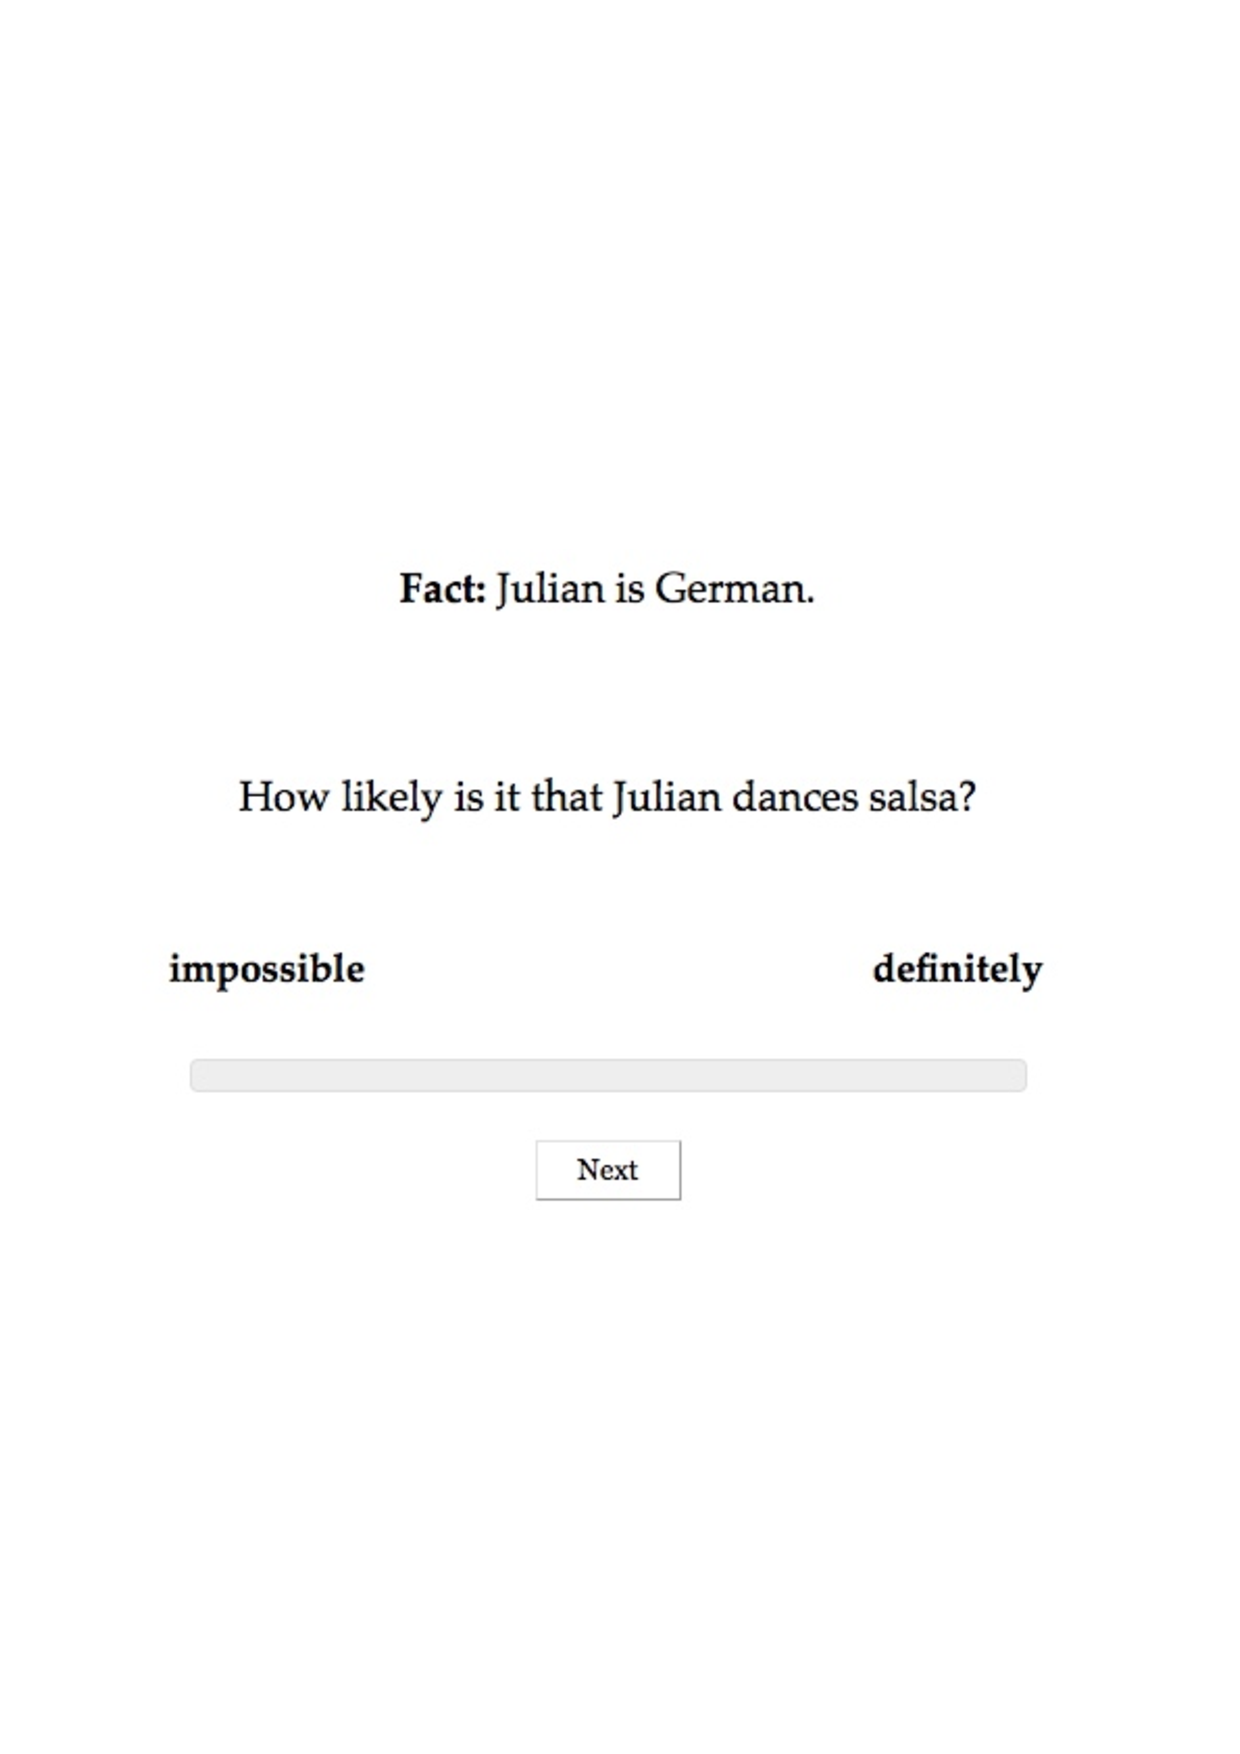
\includegraphics[width=7.6cm]{figures/exp1-prior-trial}}
\caption{Target trial in prior block (`impossible'/low prior coded as 0, `definitely'/high prior coded as 1).}\label{fig-exp1-prior}
\end{subfigure}
 \par\bigskip
\begin{subfigure}[t]{0.8\textwidth}
\par\bigskip
\centering
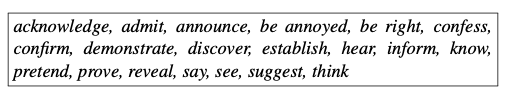
\includegraphics[width=10cm]{figures/predicates}
\caption{20 clause-embedding predicates in the at-issueness and projection blocks.}\label{fig-exp1-predicates}
 \end{subfigure}
 \par\bigskip
\begin{subfigure}[t]{0.5\textwidth}
\par\bigskip
\centering
 \fbox{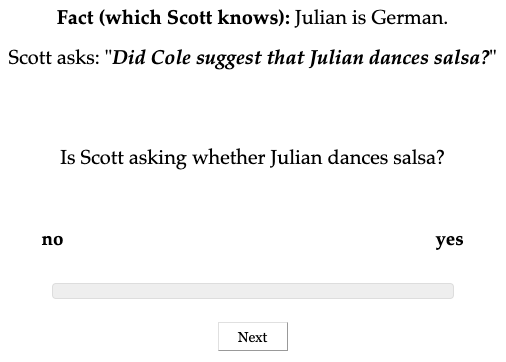
\includegraphics[width=7.6cm]{figures/exp1-nai-trial}} 
\caption{Target trial in at-issueness block (`no'/not-at-issue coded as 1, `yes'/at-issue coded as 0).}\label{fig-exp1-nai}
 \end{subfigure}%
 \hspace*{.3cm} \begin{subfigure}[t]{0.5\textwidth}
\par\bigskip
\centering
 \fbox{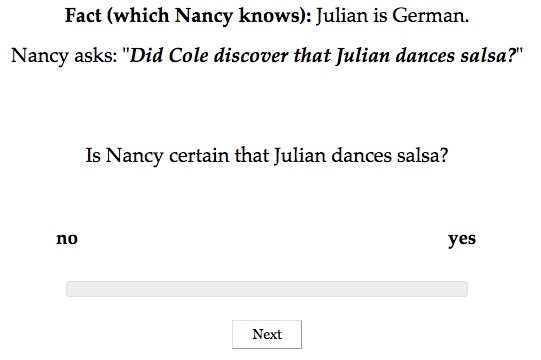
\includegraphics[width=7.6cm]{figures/exp1-projection-trial}} 
\caption{Target trial in projection block (`no'/no projection coded as 0, `yes'/projection coded as 1).}\label{fig-exp1-projection}
 \end{subfigure}

\caption{Sample target trials and clause-embedding predicates in Exp.~1.}
\end{figure}

The at-issueness and projection blocks also included 6 control trials each, which functioned as attention checks: The contents of these items were expected to be at-issue and not to project. The same 6 contents were also used to form 6 filler trials in the prior block. These filler items were not used to assess participants' attention. For the full set of control and filler items see Supplement \ref{a-stim}.

Each participant's set of items was semi-randomly generated: First, the 20 clauses were randomly paired with the 20 predicates. Then, one random half of the items was assigned the respective clause's higher-probability fact, and the other half its lower-probability fact. Participants completed a total of 78 trials: 20 target trials in each block, 6 control trials in the projection and at-issueness blocks each, and 6 filler trials in the prior block. Each participant completed the same filler and control trials.  To measure the prior probability of the contents,  the prior block was presented first to all participants. The projection and at-issueness blocks were then presented in random order. Within blocks, trial order was randomized.

After completing the experiment, participants filled out a short optional demographic survey. To encourage truthful responses, participants were told that they would be paid no matter what answers they gave in the survey.

\paragraph{Data exclusion.} Data was excluded based on self-declared non-native speaker status and other criteria shown in Supplement \ref{a-excl}, leaving 10,100 data points from 505 participants (ages 20-73; mean age: 39.5).

\subsection{Statistical analyses}\label{s:stats1}

To address the research questions in (\ref{questions}), we want to know for each lexical meaning (contributed by a clause-embedding predicate) whether there is an effect of prior probability on projection (research question I), whether there is an effect of at-issueness on projection (research question II), whether there is an effect of the interaction of prior probability and at-issueness on projection (research question IIIa), and whether there is an effect of prior probability on at-issueness (research question IIIb). To address these questions, we fit two types of models to the data. All analyses were conducted in R (\citealt{R}, version 4.3.1) using RStudio (version 2023.12.0+369).

First, to address questions (I), (II) and (IIIa), we fit 20 Bayesian mixed-effects beta regression models, one for each clause-embedding predicate, using the `brms' package (\citealt{buerkner2017}). The models predicted certainty ratings\footnote{To model the certainty ratings using a beta regression, the ratings were first transformed from the interval [0,1] to the interval (0,1) using the method proposed in \citealt{smithson-verkuilen2006}. In the models for research question (IIIb), the asking-whether ratings were also transformed in this way.} (measuring projection) from a centered fixed effect of asking-whether rating (measuring at-issueness), a centered fixed effect of prior probability rating, and their interaction. Priors on all fixed effects were flat.  The models included a random by-item intercept (where an item is a complement clause) and a random by-item slope for the fixed effects of asking-whether and prior probability rating.\footnote{By-participant random effects were not included here or in the models for research question (IIIb) because each participant saw each predicate only once.} The outputs of these models are expected means and their 95\% highest posterior density intervals (HDIs).\footnote{Since beta distributions include both a mean  ($\mu$) and precision parameter  ($\phi$), the model outputs also included expected precisions and their 95\% HDIs. However, for our purposes only  the means of the posterior distributions were relevant, so we didn't analyze the precisions.} Full model outputs are provided in the repository for Exp.~1.

Second, to address question (IIIb), we also fit 20 Bayesian mixed-effects beta regression models, one for each clause-embedding predicate. The models predicted asking-whether ratings (measuring at-issueness) from a centered fixed effect of prior probability rating, again with a flat prior on the fixed effect. The models included a random by-item intercept (where an item is a complement clause) and a random by-item slope for the fixed effect of prior probability rating. As with the models described above, the outputs of these models are expected means and 95\% highest posterior density intervals. Full model outputs are provided in the repository for Exp.~1.

To facilitate interpretation, the models did not include a fixed effect of block or an interaction between a fixed effect of block and the other fixed effects. To investigate the role of block order, we conducted auxiliary analyses on the two subsets of the data that differ in whether the projection block preceded the at-issueness block (referred to as the `proj/ai' subset) or followed it (the `ai/proj' subset). (Recall that the prior block always came first.) 

Hypothesis testing was conducted to investigate the effects of interest, that is (I) whether there was an effect of prior beliefs on projection for each of the clause-embedding predicates/lexical meanings, (II) whether there was an effect of at-issueness on projection for each of the clause-embedding predicates/lexical meanings, (IIIa), whether there was an effect of the interaction between prior beliefs and at-issueness on projection for each  for each of the clause-embedding predicates/lexical meanings, and (IIIb) whether there was an effect of prior beliefs on at-issueness for each of the clause-embedding predicates/lexical meanings. Table \ref{t:resultsExp1} reports, for each of the four hypotheses, whether there was evidence for an effect, whether the effect was positive or negative, and the Bayes factor associated with the effect. 

\subsection{Results and discussion}\label{s-results-exp1}

Fig.~\ref{fig:results1} shows participants' ratings for the full dataset. The corresponding figures for the two subsets `proj/ai' and `ai/proj' are provided in Supplement \ref{a-blockOrderExp1}.

\begin{figure}[h!]
\centering
\begin{subfigure}[t]{0.49\textwidth}
\centering
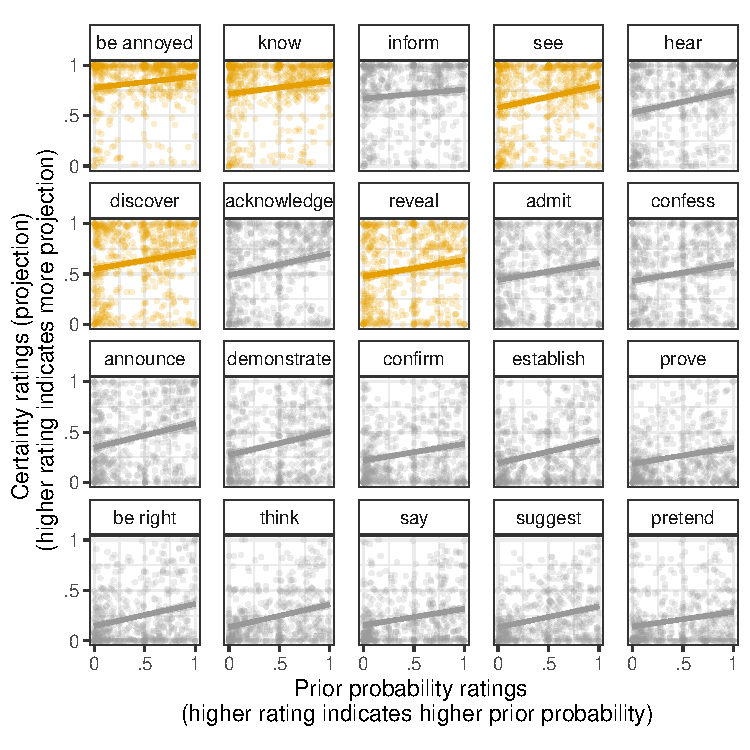
\includegraphics[width=\textwidth]{../../results/exp1/graphs/projection-by-prior}
\caption{Certainty against prior probability ratings.}\label{fig:certainty-by-prior}
\end{subfigure} \hfill \begin{subfigure}[t]{0.49\textwidth}
\centering
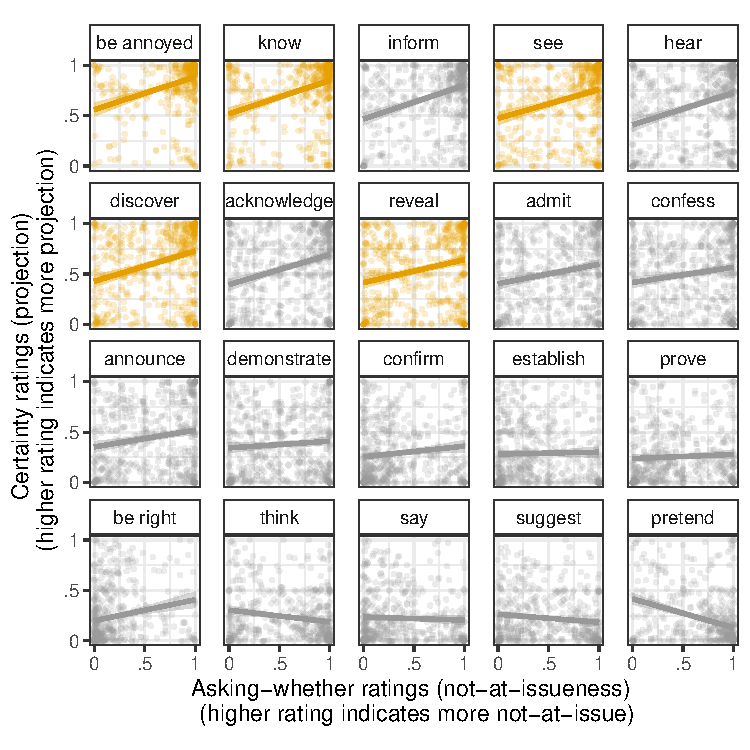
\includegraphics[width=\textwidth]{../../results/exp1/graphs/projection-by-ai}
\caption{Certainty against asking-whether ratings.}\label{fig:certainty-by-nai}
 \end{subfigure}
 
\begin{subfigure}[t]{0.49\textwidth}
\centering
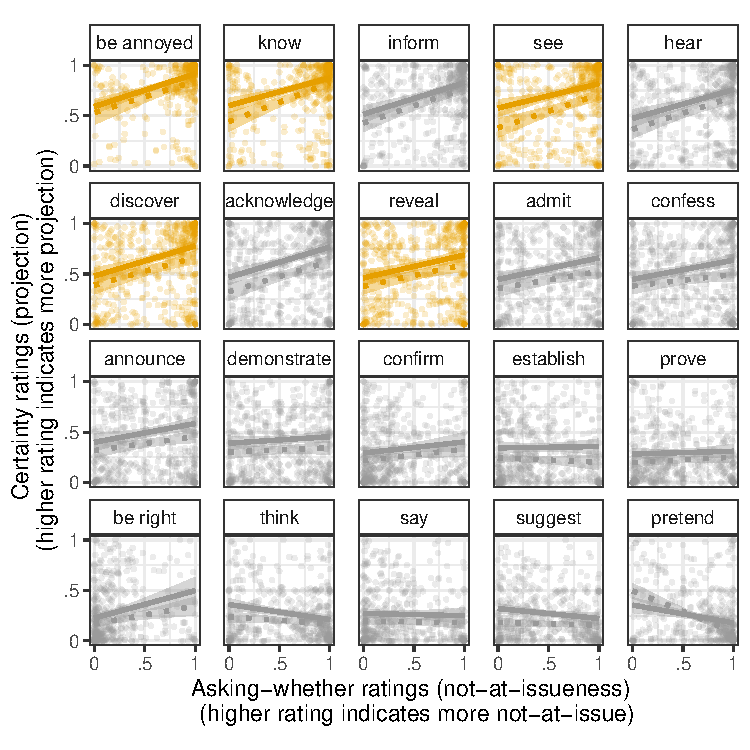
\includegraphics[width=\textwidth]{../../results/exp1/graphs/projection-by-ai-and-prior}
\caption{Certainty against asking-whether ratings by high prior probability fact (solid line: ---) and low prior probability fact (dotted line: \raisebox{1mm}{\ldots}).}\label{fig:certainty-by-ai-and-prior}
 \end{subfigure}\hfill 
\begin{subfigure}[t]{0.49\textwidth}
\centering
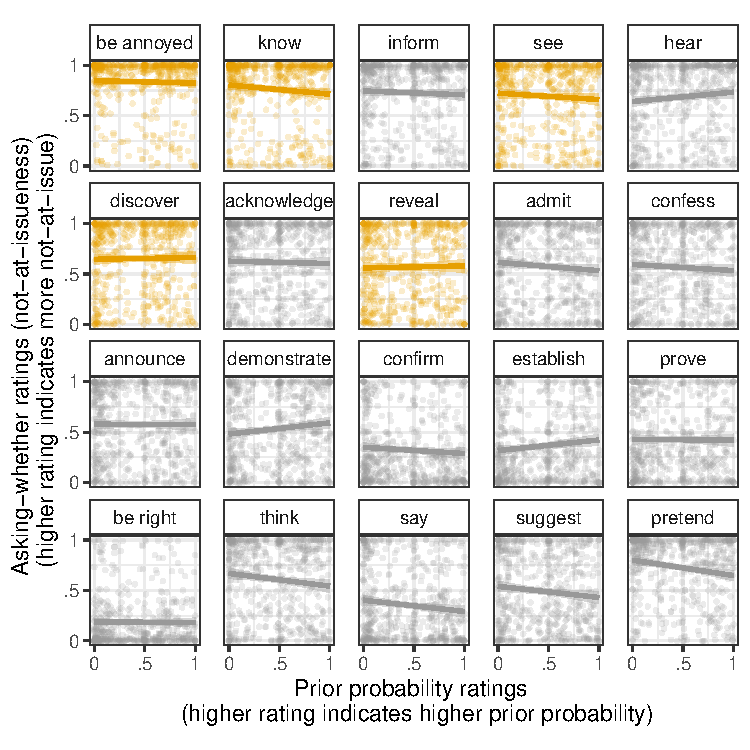
\includegraphics[width=\textwidth]{../../results/exp1/graphs/ai-by-prior}
\caption{Asking-whether against prior probability ratings.}\label{fig:ai-by-prior}
\end{subfigure} 
  
\caption{Participants' ratings in Exp.~1 (full dataset) by predicate: (a) certainty ratings (measuring projection) against prior probability ratings, (b) certainty ratings (measuring projection) against asking-whether ratings (measuring projection), (c) certainty ratings (measuring projection) against asking-whether ratings (measuring at-issueness) by high and low prior probability fact, (d) asking-whether ratings (measuring at-issueness) against prior probability ratings. Predicates are ordered by projection mean, with purportedly factive predicates in orange.}\label{fig:results1}
\end{figure}

\paragraph{(I) The relation between prior beliefs and lexical meaning in modulating projection.} Recall that \citealt{degen-tonhauser-openmind} observed a positive effect of prior probability on projection: The higher an interpreter's prior belief in a content, the more the interpreter takes the speaker to believe in the content. This result was replicated in the current experiment: As shown in Fig.~\ref{fig:certainty-by-prior}, which shows participants' certainty ratings (measuring projection) against their prior probability ratings by clause-embedding predicate,\footnote{The predicates are ordered in Figs.~\ref{fig:results1} and \ref{fig:results2} by the strength of the projection of the CC in the respective experiment.} there was a positive effect of prior for each predicate. This suggests that the more likely interpreters are to believe a content a priori, the more that content projects.

These observations were supported by the models fitted to the full dataset and to the `proj/ai' subset: As shown in Table \ref{t:resultsExp1}, there is at least strong evidence for a positive effect of prior probability on certainty ratings (measuring projection) for each predicate in the full dataset as well as in the proj/ai subset. In the ai/proj subset, there is at least strong evidence for a positive effect for 14 of the 20 predicates. However, for 4 predicates, namely {\em discover, acknowledge, reveal} and {\em say}, there is only weak to moderate evidence for a positive effect. Furthermore, there is no evidence for an effect for {\em be annoyed} and weak to moderate evidence for a negative effect for {\em inform}. 

One possible explanation for this difference between the `proj/ai' and `ai/proj' datasets is that the effect of prior beliefs on projection is an artifact of the within-participant design of Exp.~1. On this explanation, participants' certainty ratings on the projection block were artificially influenced by their prior belief ratings, but only when the prior block immediately preceded the projection block. Another possible explanation is that the effect of prior beliefs on projection is real, but when the at-issueness block directly precedes the projection block, participants' attention is drawn to the question of what the speaker is asking about, thereby drawing resources away from integrating information from the prior. One way of distinguishing these explanations is to collect certainty ratings from a set of participants who do not provide prior belief ratings and to use a separate group's prior belief ratings as a predictor of these certainty ratings. This is what we did in Exp.~2,  reported in the next section. Preliminary support for the latter explanation comes from \citepos{degen-tonhauser-openmind} Exp.~2, which suggested that there is an effect of prior beliefs on projection even when the prior belief ratings are collected from a different set of participants than the certainty ratings.
                          
\paragraph{(II) The relation between at-issueness and lexical meaning in modulating projection.} Recall that \citepos{tbd-variability} Gradient Projection Principle leads us to expect a positive effect of not-at-issueness on projection for all predicates. \citealt{djaerv-bacovcin-salt27,djaerv-bacovcin2020} and \citealt{mahler-etal2020}, on the other hand, lead us to expect a positive effect only for factive predicates and either the opposite or no effect for nonfactive ones. Fig.~\ref{fig:certainty-by-nai} shows participants' certainty ratings (measuring projection) against asking-whether ratings (measuring at-issueness) by clause-embedding predicate: There was a positive effect for most predicates (e.g., {\em know, inform, announce, acknowledge}), which suggests that for these predicates, the more not-at-issue the embedded content is, the more it projects. There was a negative effect for other predicates (e.g., {\em pretend, think}). Finally, there was no evidence for an effect of not-at-issueness on certainty ratings for a third group of predicates (e.g., {\em prove, confirm}). These observations suggest that there is by-predicate variation in the effect of at-issueness on projection.

The observations were supported by the models. As shown in Table \ref{t:resultsExp1}, there was very strong to extreme evidence for a positive effect of asking-whether rating (measuring at-issueness) on certainty ratings (measuring projection) for 13 of the 20 predicates in the full dataset and the two subsets, namely {\em be annoyed, know, inform, see, hear, discover, acknowledge, reveal, confess, admit, announce, confirm} and {\em be right}. For {\em demonstrate}, there was very strong to extreme evidence for a positive effect in the full dataset and the proj/ai subset, but no evidence for an effect in the ai/proj dataset. This suggests that, for these 14 predicates, the more not-at-issue the CC is, the more it projects. 

For {\em think, suggest} and {\em pretend}, there was at least strong evidence for a negative effect of at-issueness on projection in the full dataset, though the three predicates differed in the strength of this evidence in the two subsets: For {\em suggest} it was merely weak to moderate in both subsets, for {\em think} it was weak to moderate in one subset and very strong to extreme in the other, and it was very strong to extreme in both subsets for {\em pretend}. This suggests that, for {\em pretend, think} and possibly also {\em suggest}, the more at-issue the CC is, the more it projects. For the remaining 3 predicates ({\em establish, prove, say}), the models fit to the three datasets only provided at most weak to moderate evidence for a (positive or negative) effect of at-issueness in the full dataset, and no clear support in the two subsets. This suggests that, for these 3 predicates, there is no effect of at-issueness on projection.

These results are not predicted by \citepos{tbd-variability} Gradient Projection Principle, which does not lead us to expect predicates with negative or no effects. The results also do not entirely match the results of \citealt{djaerv-bacovcin-salt27,djaerv-bacovcin2020} and  \citealt{mahler-etal2020}: Although there was a positive effect for factive predicates, as well as a negative or no effect for some nonfactive predicates, there were also several nonfactive predicates with a positive effect (e.g., {\em inform, acknowledge, confess, admit}). 


\paragraph{(IIIa) The relation between prior beliefs and at-issueness in modulating projection.} Recall that most projection analyses in the RSA framework assume no relation between prior beliefs and at-issueness in modulating projection, that is, they assume that prior beliefs and at-issueness independently modulate projection. Fig.~\ref{fig:certainty-by-ai-and-prior} shows participants' certainty ratings (measuring projection) against asking-whether ratings (measuring at-issueness) by prior probability and by predicate. There does not seem to be an interaction for most predicates (e.g., {\em be annoyed, discover}), but some predicates seem to exhibit an interaction (e.g., {\em see, pretend}).\footnote{Whereas Fig.~\ref{fig:certainty-by-ai-and-prior} groups the prior belief ratings by the binary prior probability classification that was used to create the stimuli (higher vs.\ lower prior probability), the models  do not assume this classification because participants' prior belief ratings may not align with this binary classification. The same holds for Fig.~\ref{fig:certainty-by-ai-and-priorExp2} and the models fit to the Exp.~2 data.}

The models fit to the full dataset and the two subsets did not support the assumption of a systematic relation between prior beliefs and at-issueness in modulating projection. As shown in Table \ref{t:resultsExp1}, there was at most weak to moderate evidence for an effect of the interaction in all three datasets for 12 of the 20 predicates (namely {\em know, discover, reveal, admit, confess, announce, demonstrate, confirm, establish, prove, think, suggest}). For five predicates, there was strong to extreme evidence for an effect in one of the three datasets, but at most weak to moderate evidence in the other two ({\em inform, acknowledge, be right}) or very strong to extreme evidence for an effect of the opposite polarity in another dataset ({\em be annoyed, hear}).  Thus, for 17 of the 20 predicates, the data do not support the assumption of a systematic relation between prior beliefs and at-issueness in modulating projection. The only three predicates for which the models support the assumption of an effect are {\em see} (at least strong evidence for a negative effect in the full dataset and one subset), {\em say} (strong evidence for a positive effect in the full dataset and one subset), and {\em pretend} (at least strong evidence for a positive effect in all three datasets). 

These results provide some support for the assumption made in extant RSA models that there is no relation between prior beliefs and at-issueness in modulating projection (\citealt{qing-etal2016,stevens-etal2017,warstadt2022,pan-degen2023}). However, if the effects for {\em see, say} and {\em pretend} replicate in Exp.~2, such analyses will need to allow for individual predicates to exhibit an interaction between prior beliefs and at-issueness in modulating projection.

\paragraph{(IIIb) The relation between prior beliefs and at-issueness.} 

Recall that \citepos{tonhauser-etal-eval} Non-redundancy Principle for At-issue Content predicts a positive effect of prior beliefs on not-at-issueness. With respect to Fig.~\ref{fig:ai-by-prior}, which shows participants' asking-whether ratings (measuring at-issueness) by their prior probability ratings, this principle leads us to expect a positive effect for all of the predicates. While there may be a weakly positive effect for {\em hear} and {\em demonstrate}, there does not seem to be a effect for many of the 20 predicates, and a negative one for {\em think, say, suggest} and {\em pretend}.

These observations were supported by the models. As shown in Table \ref{t:resultsExp1}, there was either no evidence for an effect of prior beliefs on at-issueness or only weak to moderate evidence in all three datasets for 8 of the 20 predicates (namely {\em inform, see, discover, acknowledge, reveal, admit, announce, be right}). For {\em hear} and {\em demonstrate}, there was at last strong evidence for a positive effect of prior beliefs on at-issueness in the full dataset and one of the subsets. For {\em be annoyed, know, admit, think, say, suggest} and {\em pretend}, there was at least strong evidence for a negative effect in the full dataset and one of the two subsets. These results suggest that the effect of prior beliefs on at-issueness exhibits by-predicate variation. That there was either no evidence for an effect or at least strong evidence for a negative effect for 15 of the 20 predicates does not support \citepos{tonhauser-etal-eval} Non-redundancy Principle for At-issue Content., which predicts a positive effect across the board.


\setlength{\fboxrule}{0pt}

\begin{table}[h!]
\begin{subtable}[h]{1\textwidth}
\setlength{\tabcolsep}{3pt}
\centering
\input{../../results/exp1/models/latex-tables/t1}
\caption{Results of Exp.~1}\label{t:resultsExp1}
\end{subtable}

\vspace*{.4cm}

\begin{subtable}[h]{1\textwidth}
\setlength{\tabcolsep}{3.5pt}
\centering
\input{../../results/exp2/models/latex-tables/t1}
\caption{Results of Exp.~2}\label{t:resultsExp2}
\end{subtable}

\caption{Summary of the results of Exps.~1 and 2. The `Effect' column identifies the research question and the hypothesized effect, and the `Data' column whether the model was fit to the full dataset (`full') or a subset with a particular block order ('proj/ai', 'ai/proj'). Predicates are ordered by mean projection in Exp.~1 with factive predicates in \color{orange}orange\color{black}. Color coding indicates whether the effect was positive (red) or negative (blue), and the Bayes factor associated with the effect: \colorbox{red1}{\makebox[1em][c]{\framebox[1em]{\rule{0pt}{3pt}}}},\colorbox{blue1}{\makebox[1em][c]{\framebox[1em]{\rule{0pt}{3pt}}}}: 21+ (``very strong to extreme evidence''), 
\colorbox{red2}{\makebox[1em][c]{\framebox[1em]{\rule{0pt}{3pt}}}},\colorbox{blue2}{\makebox[1em][c]{\framebox[1em]{\rule{0pt}{3pt}}}}: 11-20 (``strong evidence''), 
\colorbox{red4}{\makebox[1em][c]{\framebox[1em]{\rule{0pt}{3pt}}}},\colorbox{blue4}{\makebox[1em][c]{\framebox[1em]{\rule{0pt}{3pt}}}}: 2-10 (``weak to moderate evidence'').
White indicates that there was no evidence for an effect. 
}

\end{table}

%
%
%\subsection{Discussion}\label{s:discussion-exp1}
%
%The results of Exp.~1 replicate the results of prior research, namely that that prior beliefs, at-issueness, and lexical meaning modulate projection. Crucially, the results provide insight into the relations between these factors. 
%
%Regarding (I) the relation between prior beliefs and lexical meaning in modulating projection, the model fit to the full dataset suggests that there is an effect of prior beliefs on projection that persists across the lexical meanings of the 20 clause-embedding predicates. While this effect came out in the subset of the data in which the projection block immediately followed the prior block, it did not in the subset of the data in which the at-issueness block intervened between the prior block and the projection block. One possible explanation is that the effect of prior beliefs on projection is an artifact of the design of Exp.~1, such that participants' certainty ratings on the projection block are artificially influenced by their prior belief ratings, but only when the prior blick immediately precedes the projection block. Another possible explanation is that the effect of prior beliefs on projection is real, but when the at-issueness block directly precedes the projection block, participants' attention is drawn to the question of what the speaker is asking about, thereby drawing resources away from integrating information from the prior. One way of distinguishing these explanations is to collect certainty ratings from a set of participants who did not also provide prior belief ratings and using a separate group's prior belief ratings as a predictor of these certainty ratings. This is what we will do in Exp.~2, which is reported on in the next section. Preliminary support for the latter explanation comes from \citepos{degen-tonhauser-openmind} Exp.~2, which suggested that there is an effect of prior beliefs on projection even when the prior belief ratings were collected from a different set of participants than the projection ratings (but the contribution of lexical meaning was not considered in that work).
%
%Regarding (II) the relation between at-issueness and lexical meaning in modulating projection, the models fit to the full dataset and the two subsets suggest that there is a systematic effect of at-issueness on projection for some predicates. Specifically, for {\em acknowledge, admit, announce,  be annoyed, be right, confess, discover, hear, establish, inform, know, reveal} and {\em see}, Exp.~1 suggests that the more not-at-issue the CC of these predicates is, the more it projects. This result is not in line with \citepos{djaerv-bacovcin2020} analysis, as it leads us to expect this relation only for factive predicates, not for nonfactive ones. While the results for these predicates are in line with \citepos{tbd-variability} Gradient Projection Principle, there are also predicates whose lexical meaning does not appear to interact with at-issueness in the way that is expected from the Gradient Projection Principle. The lexical meaning of {\em pretend}, for instance, appears to interact with at-issueness in the opposite way, such that the more not-at-issue the CC is, the less it projects; this is also suggested for {\em think} and {\em suggest}, at least by the model fit to the full dataset and the subset in which the at-issueness block follows the projection block. And the lexical meaning of predicates like {\em confirm, demonstrate, establish, prove}, and {\em say} appears to only show the effect expected by the Gradient Projection Principle when the at-issueness block follows the projection block. To understand whether these interactions between lexical meaning and at-issueness replicate, we ran Exp.~2. A discussion of the theoretical implications of the results is postponed to section \ref{s4}.
%
%Finally, regarding (III) the relation between prior beliefs and at-issueness, the analyses of the entire dataset of Exp.~1 and of the two subsets suggests that these two factors do not interact in modulating projection. This result is in line with what is assumed in extant RSA models of projection inferences (\citealt{qing-etal2016,stevens-etal2017,warstadt2022,pan-degen2023}) and contrary to \citepos{tonhauser-etal-eval} Non-redundancy Principle for At-issue Content, which assumed that the higher the a priori belief in a content is, the less at-issue it is. 

\section{Experiment 2}\label{s3}

The results of Exp.~1 provide novel insight into the relation between prior beliefs, at-issueness and lexical meaning in modulating projection inferences, as well as into the relation between prior beliefs and at-issueness. But the result addressing research question (I) also raised the question of whether the effect of prior beliefs on projection is real or merely an artifact of the within-participant design of Exp.~1. Exp.~2 was designed to investigate this open question: its design was identical to that of Exp.~1, except that there was no prior block. To investigate the relation between prior beliefs, at-issueness, and lexical meaning in modulating projection inferences, we added to the data collected in Exp.~2 the mean prior probability ratings of the 40 content/fact combinations collected in three previous experiments, namely Exp.~1, the prior block of Exp.~1 in \citealt{degen-tonhauser-openmind}, and Exp.~2a in \citealt{degen-tonhauser-openmind}. Exp.~2 also allows us to investigate whether the results obtained for research questions (II), (IIIa) and (IIIb) replicate.  

\subsection{Methods}

\paragraph{Participants.} 600 participants with U.S.\ IP addresses and at least 99\% of previous HITs approved were recruited on Amazon's Mechanical Turk platform (ages: 19-73, median: 37.5). They were paid \$2.20.\footnote{92 individuals participated in both Exp.~1 and Exp.~2. Since the experiments were run four months apart (Exp.~1: December 16, 2019; Exp.~2: August 21, 2019), it is unlikely that these participants' responses were primed by their prior participation.}

\paragraph{Materials and procedure.}  Exp.~2 differed from Exp.~1 only in that there was no prior block. As in Exp.~1, each participant's set of items was semi-randomly generated: First, the 20 clauses were randomly paired with the 20 predicates. Then, one random half of the items was assigned the respective clause's higher-probability fact, and the other half its lower-probability fact. Participants completed a total of 52 trials: 20 target trials in each block, and 6 control trials in the projection and at-issueness blocks each. Each participant completed the same control trials. The projection and at-issueness blocks were presented in random order. 

\paragraph{Data exclusion.} Data was excluded based on self-declared non-native speaker status and other criteria shown in Supplement \ref{a-excl}, leaving 10,160 data points from 508 participants (ages 19-73; mean age: 38.3).

\subsection{Statistical analyses}

To address the research questions in (\ref{questions}), we fit the same two types of models to the data as in Exp.~1 (see section \ref{s:stats1}). However, in contrast to the models for Exp.~1, where there was a centered fixed effect of prior probability rating, there was a centered fixed effect of {\em mean} prior probability rating in the models for Exp.~2. This is because the prior probability ratings were aggregated by content/fact combination, as they came from a different set of participants than the participants of Exp.~2. The outputs of these models are expected means and 95\% highest posterior density intervals. Full model outputs are provided in the repository for Exp.~2.

Hypothesis testing was conducted to investigate the effects of interest, that is (I) whether there was an effect of mean prior beliefs on projection for each of the clause-embedding predicates/lexical meanings, (II) whether there was an effect of at-issueness on projection for each of the clause-embedding predicates/lexical meanings, (IIIa), whether there was an effect of the interaction between mean prior beliefs and at-issueness on projection for each  for each of the clause-embedding predicates/lexical meanings, and (IIIb) whether there was an effect of mean prior beliefs on at-issueness for each of the clause-embedding predicates/lexical meanings. Table \ref{t:resultsExp2} reports, for each of the four hypotheses, whether there was evidence for an effect, whether the effect was positive or negative, and the Bayes factor of the evidence. 

\subsection{Results and discussion}

Fig.~\ref{fig:results2} shows participants' ratings for the full dataset. The corresponding figures for the two subsets `proj/ai' and `ai/proj' are provided in Supplement \ref{a-blockOrderExp2}.


\begin{figure}[h!]
\centering
\begin{subfigure}[t]{0.49\textwidth}
\centering
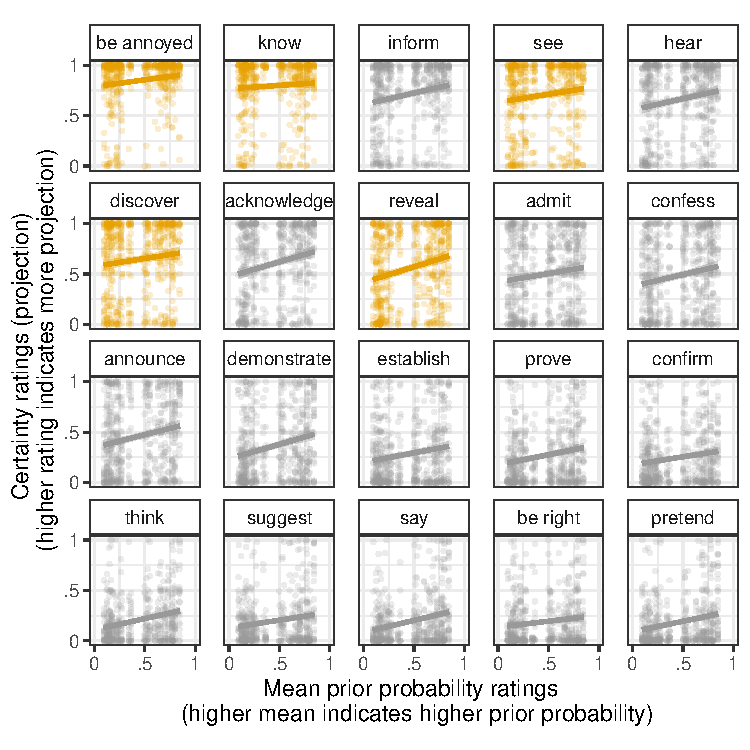
\includegraphics[width=\textwidth]{../../results/exp2/graphs/projection-by-prior}
\caption{Certainty against mean prior probability ratings.}\label{fig:certainty-by-priorExp2}
\end{subfigure} \hfill \begin{subfigure}[t]{0.49\textwidth}
\centering
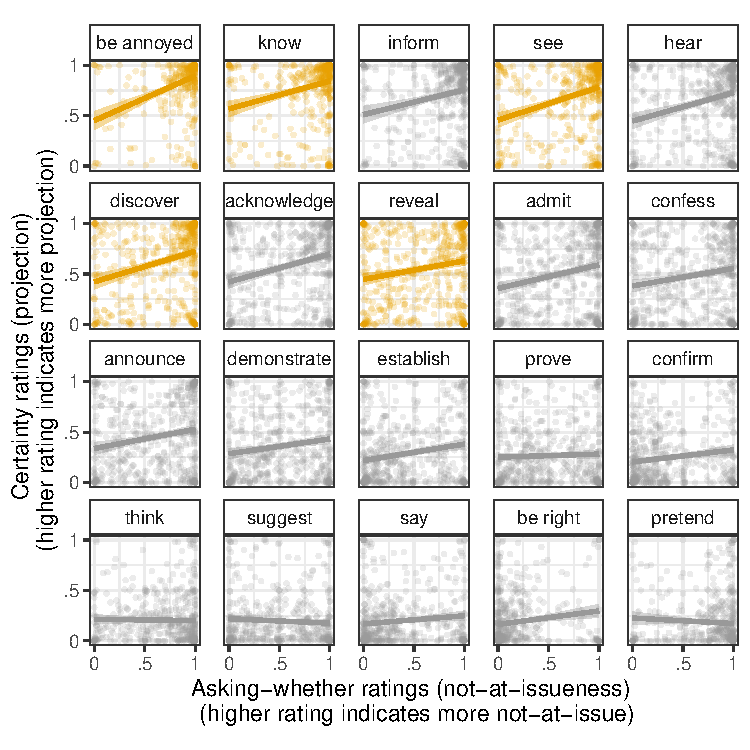
\includegraphics[width=\textwidth]{../../results/exp2/graphs/projection-by-ai}
\caption{Certainty against asking-whether ratings.}\label{fig:certainty-by-naiExp2}
 \end{subfigure}
 
\begin{subfigure}[t]{0.49\textwidth}
\centering
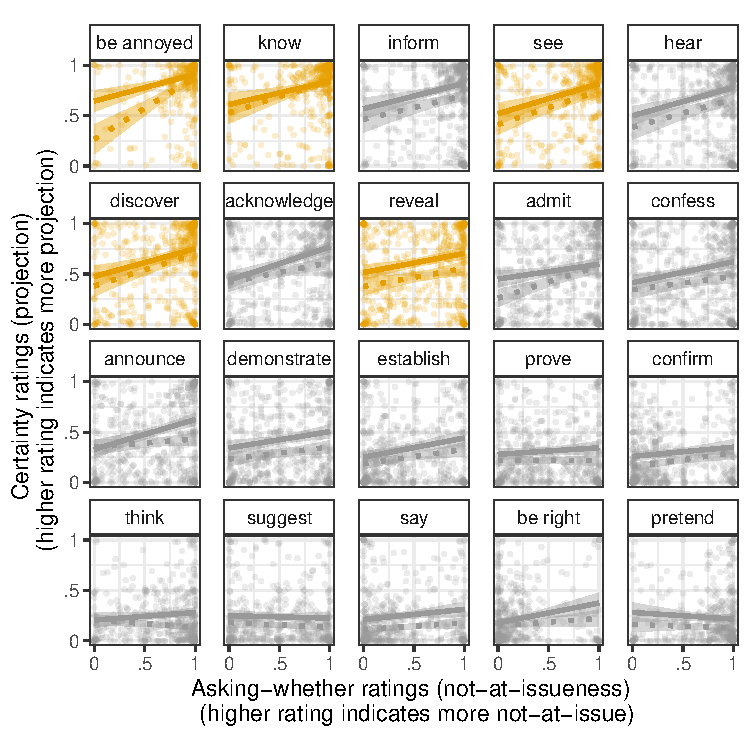
\includegraphics[width=\textwidth]{../../results/exp2/graphs/projection-by-ai-and-prior}
\caption{Certainty against asking-whether ratings by higher prior probability fact (solid line: ---) and lower prior probability fact (dotted line: \raisebox{1mm}{\ldots}).}\label{fig:certainty-by-ai-and-priorExp2}
 \end{subfigure}\hfill 
\begin{subfigure}[t]{0.49\textwidth}
\centering
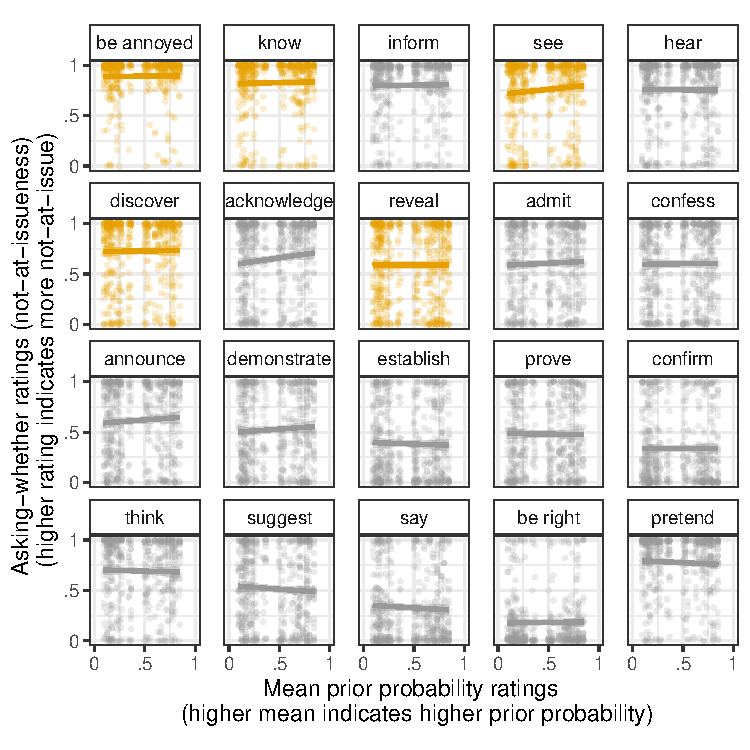
\includegraphics[width=\textwidth]{../../results/exp2/graphs/ai-by-prior}
\caption{Asking-whether against mean prior probability ratings.}\label{fig:ai-by-priorExp2}
\end{subfigure} 
  
\caption{Participants' ratings in Exp.~2 (full dataset) by predicate: (a) certainty ratings (measuring projection) against mean prior probability ratings, (b) certainty ratings (measuring projection) against asking-whether ratings (measuring projection), (c) certainty ratings (measuring projection) against asking-whether ratings (measuring at-issueness) by higher and lower prior probability fact, (d) asking-whether ratings (measuring at-issueness) against mean prior probability ratings. Linear smoothers with 95\% confidence intervals overlaid. Predicates are ordered by projection mean in Exp.~2, with purportedly factive predicates in orange.}\label{fig:results2}
\end{figure}

\paragraph{(I) The relation between prior beliefs and lexical meaning in modulating projection.}  Fig.~\ref{fig:certainty-by-priorExp2} shows, for each predicate, participants' certainty ratings for the content/fact combinations against the mean prior probability ratings for the content/fact combinations that were collected from a different set of participants. There is a positive effect for each predicate. These observations were supported by the models fit to the full dataset and for the `proj/ai' dataset. As shown in Table \ref{t:resultsExp2}, there was at least strong evidence for a positive effect of mean prior probability ratings on certainty ratings (measuring projection) for each predicate in the full dataset as well as in the proj/ai subset (except for {\em admit}, where the evidence was weak to moderate). In the ai/proj subset, the evidence was merely weak to moderate for a positive effect for {\em see, discover, announce, confirm} and {\em be right}, and for a negative effect for {\em know}. 

 These results suggest that the effect of prior beliefs on projection observed in Exp.~1 was not an artifact of the within-participant design of that experiment. Rather, the results of Exps.~1 and 2 together support the assumption that participants integrate their prior beliefs about content when providing certainty ratings, regardless of whether they were asked to give prior probability ratings in an earlier block (Exp.~1) or not (Exp.~2). The fact that in both Exps.~1 and 2 the evidence for a positive effect of prior beliefs on projection is weaker in the `ai/proj' block than in the `proj/ai' block further suggests that when participants' attention is drawn to the question of what the speaker is asking about, integrating information from their prior beliefs into their certainty ratings is more challenging than if they give certainty ratings before giving asking-whether ratings. Overall then, the results of Exps.~1 and 2 support the hypothesis that participants' prior beliefs about content modulate their projection ratings for each of the 20 predicates under investigation.
                          
\paragraph{(II) The relation between at-issueness and lexical meaning in modulating projection.}  Recall, again, that \citepos{tbd-variability} Gradient Projection Principle predicts a positive effect of not-at-issueness on projection for all predicates. \citealt{djaerv-bacovcin-salt27,djaerv-bacovcin2020} and \citealt{mahler-etal2020}, on the other hand, predict a positive effect only for factive predicates and either the opposite or no effect for nonfactive ones. Fig.~\ref{fig:certainty-by-naiExp2} shows participants' certainty ratings (measuring projection) against asking-whether ratings (measuring not-at-issueness) by clause-embedding predicate: There was a positive effect of not-at-issueness on projection for most predicates (e.g., {\em know, inform, announce, acknowledge}). There were also predicates with no effect (e.g., {\em think, suggest, pretend}). In contrast to Exp.~1, there were no predicates with a clearly negative effect. 

These observations were supported by the models. There was at least strong evidence for a positive effect of asking-whether rating (measuring at-issueness) on certainty ratings (measuring projection) for 12 of the 20 predicates in the full dataset and the two subsets: {\em be annoyed, know, inform, see, hear, discover, acknowledge, admit, confess, announce, demonstrate} and {\em confirm}. For an additional 5 predicates, there was at least strong evidence for a positive effect in the full dataset, and at least strong evidence in one of the subsets:  {\em reveal, establish, prove, be right} and {\em say}. This suggests that, for these 17 predicates, the more not-at-issue the CC is, the more it projects. The models supported the assumption of a negative effect of projection on at-issueness only for {\em suggest}, where there was very strong to extreme evidence for a negative effect in the full dataset and in the `ai/proj' subset. For {\em think} and {\em pretend}, the results of Exp.~2 did not support the assumption of an effect of at-issueness on projection. These observations again suggest that there is by-predicate variation in the effect of at-issueness on projection, though the variation is not identical to that of Exp.~1. 

Comparing the results of Exp.~2 to those of Exp.~1, we found evidence for a positive effect of at-issueness on projection in both experiments for 14 predicates, namely {\em be annoyed, know, inform, see, hear, discover, acknowledge, reveal, admit, confess, announce, demonstrate, confirm} and {\em be right}. These predicates include those with the highest certainty ratings (that is, the predicates whose CCs are most projective), but also \emph{be right}, a predicate whose CC is only weakly projective. Among the remaining six predicates, there were two for which the polarity of the effect of at-issueness on projection was the same across the two experiments, but stronger in Exp.~2 than Exp.~1, namely {\em prove} (positive effect) and {\em suggest} (negative effect). For the remaining 4 predicates ({\em establish, think, say, pretend}), the results of Exp.~1 did not replicate in Exp.~2, as either the polarity of the effect changed between the two experiments, or there was no effect in Exp.~2. 

Overall, then, we take the results of Exps.~1 and 2 to suggest that there is by-predicate variation in the effect of at-issueness on projection: For 14 of the 20 predicates, the CC is more projective when it is more not-at-issue. For {\em suggest}, the CC is more projective when it is less at-issue. And for the remaining 5 predicates (\emph{think, pretend, establish, say, prove}) there is no consistent effect of at-issueness on projection across the two experiments. These results  are not completely predicted by the Gradient Projection Principle (which does not lead us to expect predicates without a positive effect). The results also do not entirely match the results of \citealt{djaerv-bacovcin-salt27,djaerv-bacovcin2020}, who did not observe nonfactive predicates with positive effects or verbal nonfactive predicates with no effects, or the results of \citealt{mahler-etal2020}, who did not not observe nonfactive predicates with positive effects.

What are the relevant properties of the six predicates which did not display a positive effect of at-issueness on projection (\emph{suggest, think, pretend, establish, say, prove})? As noted above, it is not appropriate to characterize these predicates as having weakly projective CCs because the CC of {\em be right} is on par with these predicates when it comes to projection, but does exhibit an effect of at-issueness on projection (see Supplement \ref{a-proj-by-ai} for a visualization). For three of these predicates, namely \emph{pretend, think} and \emph{suggest}, we hypothesize that they do not show a positive effect of at-issueness on projection because their lexical meanings facilitate an inference that the speaker does not believe that the CC is true. This is most easily motivated for {\em pretend}, which lexically entails that the CC is false (\#\emph{Cole is pretending that Julian dances salsa, and Julian (indeed) dances salsa}). For \emph{think} and {\em suggest}, in turn, it is plausible that utterances with these predicates may give rise to the scalar implicature that the speaker does not believe the CC to be true by virtue of the speaker not having used \emph{know}, the stronger alternative that entails that the speaker believes the CC to be true. Thus, even though the CCs of these predicates are at least moderately not-at-issue in both Exps.~1 and 2 (see Supplement \ref{a-proj-by-ai}), the CC is not equally projective due to the lexical meanings of these predicates.

Unlike \emph{suggest, think}, and \emph{pretend}, the predicates \emph{establish, say}, and \emph{prove} cannot plausibly be taken to contribute to an inference that the speaker does not believe that the CC is true. These three predicates also differ from the other three in that Exp.~2 provided evidence for a positive effect of at-issueness on projection, but not Exp.~1. What might explain this difference between Exps.~1 and 2? An observation that may be relevant is that asking-whether ratings were not as stable across the two experiments as certainty ratings: The Spearman rank coefficient was only .72 for the mean asking-whether ratings of the 800 by-predicate/content/fact combinations, but .85 for the mean certainty ratings. (See Supplement \ref{a-replication} for details.) This might be taken to suggest that asking-whether ratings are more susceptible than certainty ratings to the ways in which participants might enrich the context in which they interpret the stimuli or to the (implicit) prosody with which they read the stimuli. If the lexical meanings of \emph{establish, say}, and \emph{prove} are such that such factors may modulate the at-issueness of the CC more than its projection, this might offer a path to an explanation of the differences in results between the two experiments.  

\paragraph{(IIIa) The relation between prior beliefs and at-issueness in modulating projection.} Fig.~\ref{fig:certainty-by-ai-and-priorExp2} shows participants' certainty ratings (measuring projection) against asking-whether ratings (measuring at-issueness) by mean prior probability and by predicate. For some predicates, there does not seem to be an interaction (e.g., {\em inform, see, hear}), while there appears to be one for others  (e.g., {\em be annoyed, admit, announce}). 

The models fit to the full dataset and the two subsets did not support the assumption of a systematic relation between prior beliefs and at-issueness in modulating projection across the 20 predicates. For 9 of the 20 predicates, there was either no evidence for an effect or only weak to moderate evidence for an effect in all three datasets (namely {\em know, see, hear, discover, reveal, demonstrate, establish, prove, pretend}). For the three predicates {\em be annoyed, confess}, and {\em suggest} the overall evidence was inconclusive.  Finally, there were 8 predicates for which there was at least strong evidence for an effect in the full dataset and one of the subsets: This effect was positive for {\em inform, acknowledge, announce, be right} and {\em think}, and negative for {\em admit, confirm} and {\em say}. While the results for these 8 predicates may be taken to suggest that there is an interaction between prior beliefs and at-issueness in modulating projection, it is important to note that none of these effects were observed in Exp.~1. Furthermore, none of the effects observed in Exp.~1 replicated in Exp.~2: Whereas the results of Exp.~1 suggested a negative effect for {\em see} and a positive effect for {\em say} and {\em pretend}, the results of Exp.~2 do not support an effect for {\em see} and {\em pretend}, and they support a negative effect for {\em say}. We therefore take the results of Exps.~1 and 2 to suggest that there is no systematic relation between prior beliefs and at-issueness in modulating projection inferences for the CCs of the 20 clause-embedding predicates we investigated. This, in turn, provides support for the assumption made in extant RSA models of projection inferences that prior beliefs and at-issueness independently modulate projection (\citealt{qing-etal2016,stevens-etal2017,warstadt2022,pan-degen2023}). 

\paragraph{(IIIb) The relation between prior beliefs and at-issueness.} 

Fig.~\ref{fig:ai-by-priorExp2}, which shows participants' asking-whether ratings (measuring at-issueness) by the mean prior probability ratings, does not suggest that there is a effect for most of the 20 predicates. (Recall that \citepos{tonhauser-etal-eval} Non-redundancy Principle for At-issue Content leads us to expect positive effects.)

This observation was supported by the models. For 15 of the 20 predicates, there was at most weak to moderate evidence for an effect of mean prior beliefs on at-issueness (namely {\em know, inform, hear, discover, reveal, confess, announce, demonstrate, confirm, establish, prove, be right, think, say, pretend}). For the remaining 5 predicates, there was at least some evidence for an effect, but none of these were observed in Exp.~1: For instance, whereas there was very strong to extreme evidence for a positive effect for {\em see} in the full dataset and the `ai/proj' subset of Exp.~2, there was at most weak to moderate evidence for a negative effect in Exp.~1. Similarly, whereas there was at least strong evidence for a positive effect for {\em acknowledge} in the full dataset and the `proj/ai' dataset of Exp.~2, there was no evidence for an effect in Exp.~1. Furthermore, none of the effects observed in Exp.~1 for {\em hear, demonstrate, be annoyed, know, admit, think, say, suggest}, and {\em pretend} replicated in Exp.~2: For all of these predicates, there was at most weak to moderate evidence for an effect of the same polarity in Exp.~2 in the full dataset. 

We suggest that the results of Exps.~1 and 2 taken together provide support for the assumption that there is no systematic effect of prior beliefs on at-issueness, contrary to the positive effect that is predicted by \citepos{tonhauser-etal-eval} Non-redundancy Principle for At-issue Content.

\section{General discussion}\label{s4}

This paper  reported the results of two experiments designed to investigate interactions between three factors that have been shown in prior research to modulate projection, namely prior beliefs, at-issueness, and lexical meaning. Taken together, the results of Exps.~1 and 2 suggest the following answers to the research questions:


\begin{exe}

\exi{{\bf (I)}} {\bf Prior beliefs and lexical meaning:} Do prior beliefs modulate projection across clause-embedding predicates, that is, across lexical meanings?

\underline{Answer:} Yes. There was a systematic effect of prior beliefs on projection across the meanings of the 20 clause-embedding predicates investigated. The greater an interpreter's prior beliefs in the CC, the more the CC is taken to project.

\exi{{\bf (II)}} {\bf At-issueness and lexical meaning:} Is content that is more not-at-issue also more projective for all clause-embedding predicates (as expected under \citepos{tbd-variability} Gradient Projection Principle) or only for factive predicates, with either the opposite or no effect for nonfactive predicates (as observed in \citealt{djaerv-bacovcin-salt27,djaerv-bacovcin2020,mahler-etal2020})? 

\underline{Answer:} There was by-predicate variation in the effect of at-issueness on projection. While the CCs of most predicates were more projective the more not-at-issue they were, there were also predicates that did not show a positive effect. This result is  not completely predicted by the Gradient Projection Principle, which does not predict a lack of positive effect for any predicate. It also differs from the results of \citealt{djaerv-bacovcin2020} and \citealt{mahler-etal2020}, who did not find a positive effect for nonfactive predicates.

\exi{{\bf (III)}} {\bf Prior beliefs and at-issueness:} 
\begin{xlist}
\exi{{\bf a.}}  Do the prior probability and at-issueness of content independently modulate projection inferences  (as assumed in most RSA models of projection inferences), or do they interact?  

\underline{Answer:} The results of Exps.~1 and 2 did not establish systematic evidence for an interaction between prior probability and at-issueness on projection.

\exi{{\bf b.}} Is content with greater a priori probability more not-at-issue (as expected under \citepos{tonhauser-etal-eval} Non-redundancy Principle for At-issue Content)?

\underline{Answer:} No. The results of Exps.~1 and 2 did not establish systematic evidence for an effect of prior probability on at-issueness. 

\end{xlist}
%\end{xlist}
\end{exe}

In the remainder of this section, we discuss whether contemporary analyses can capture (I) the systematic effect of prior beliefs on projection and (II) the by-predicate variation in the effect of at-issueness on projection. We consider analyses that are among the strongest contenders for capturing these effects, but find that none of them are fully able to do so.

\subsection{\citealt{heim83} and \citealt{djaerv-bacovcin2020}}\label{s41}

The analysis proposed in \citealt{djaerv-bacovcin2020} is an extension of \citealt{heim83}, where presuppositions are specified in the lexical entries of the triggering expressions. For clause-embedding predicates, this means that the CCs of factive predicates are lexically specified as presupposed, whereas the CCs of nonfactive predicates are not. Because presuppositions must be satisfied in the input context before the context is updated with the utterance, these analyses predict that the CCs of factive predicates project from under entailment-canceling operators, either because they are already entailed by the input context or because they are accommodated into the input context. Presuppositions are locally accommodated (in the local context of the entailment-canceling operator) only if global accommodation into the input context would result in inconsistency.

\citealt{djaerv-bacovcin2020} supplemented \citepos{heim83} analysis by proposing that prosody provides a cue to the QUD addressed by the utterance. Specifically, they proposed that utterances of clause-embedding predicates with focus on the subject of the embedded clause, as in (\ref{anna}a), give rise to the QUD inference that somebody has the property denoted by the verb phrase of the embedded clause but it is not known who. On the other hand, the variant with focus on the embedding predicate, as in (\ref{anna}b), gives rise to the QUD inference that the attitude holder has some relationship with the embedded proposition.

\begin{exe}
\ex\label{anna} \citealt[73]{djaerv-bacovcin2020}
\begin{xlist}
\ex John might've discovered that [Anna]$_F$ left town. \\ QUD inference: Somebody left town but it is not known who.
\ex John might've [discovered]$_F$ that Anna left town.  \\ QUD inference: John has some relationship with the proposition that Anna left town.
\end{xlist}
\end{exe}
\citealt{djaerv-bacovcin2020} assumed that the strength of the projection inference observed for utterances of sentences with focused clause embedding predicates, as in (\ref{anna}b), provides a baseline against which the effect of focus on the embedded subject, as in (\ref{anna}a), can be evaluated. Their analysis predicts that this effect of focus differs for factive and nonfactive predicates: For factive predicates, the QUD inference (specifically, in (\ref{anna}a), that it is not known who left town) weakens the projection inference triggered by the factive predicate (that Anna left town). For the version of (\ref{anna}a) with a nonfactive predicate, the QUD inference (specifically, that somebody left town) is taken to strengthen an inference to the truth of the CC, where no projection inference is lexically triggered by the nonfactive predicate.\footnote{The results of Exp.~1 reported on in \citealt{djaerv-bacovcin2020} support this analysis for the three verbal nonfactive predicates investigated, but not for the three adjectival nonfactive predicates, where this effect of subject focus was not observed.}

\citealt{djaerv-bacovcin2020} did not explicitly relate their analysis to at-issueness, but one might assume that the CC is at-issue in utterances of sentences in which the embedded subject is focused, as in (\ref{anna}a), whereas the CC is not-at-issue when the embedding predicate is focused, as in (\ref{anna}b). Under this interpretation,  \citepos{djaerv-bacovcin2020} extension of \citepos{heim83} analysis predicts that when the CC of a factive predicate is at-issue, it is less projective, whereas the opposite effect is expected for nonfactive predicates. We now consider whether \citealt{heim83} and \citealt{djaerv-bacovcin2020} capture the results of our experiments. 

\paragraph{(I) The relation between prior beliefs and lexical meaning in modulating projection.}
Neither analysis predicts the effect of prior beliefs on projection across the 20 clause-embedding predicates, for two reasons. The first reason is that neither analysis makes predictions about the projection of the majority of the 20 predicates, namely the 15 nonfactive ones (see \citealt{degen-tonhauser-language} for extensive discussion). The second reason is that prior beliefs do not play a role in either analysis. One could imagine an extension on which presupposition accommodation is sensitive to the strength of the prior belief in the presupposition. Specifically, one might assume that the lower the prior belief in the presupposition, the more likely is not accommodated globally, but locally. This extension would, however, constitute a major change for these analyses, where global accommodation taken to be the default, and local accommodation is only licensed if global accommodation of the presupposition leads to inconsistency.

\paragraph{(II) The relation between at-issueness and lexical meaning in modulating projection.} \citepos{djaerv-bacovcin2020} extension of \citealt{heim83} does not predict the observed by-predicate variation in the effect of at-issueness on projection. This is because our experiments suggest that greater not-at-issueness results in greater projection not just for the CCs of factive predicates but also for several nonfactive predicates. While \citepos{djaerv-bacovcin2020} analysis correctly predicts the pattern observed for factive predicates and for {\em suggest}, where we found a negative effect, they predict the opposite of what is observed for many of the nonfactive predicates we investigated (namely a negative effect where a positive one is observed).

\bigskip

In sum, \citealt{heim83} and the extension in \citealt{djaerv-bacovcin2020} correctly predict that the CCs of factive predicates project and that greater not-at-issueness leads to greater projection for these predicates. These analyses do not, however, predict that the CCs of nonfactive predicates are also projective, that greater not-at-issueness may also lead to greater projection for nonfactive predicates predicates, and they also do not predict the effect of prior beliefs on projection for the CCs of clause-embedding predicates.

\subsection{\citealt{abrusan2011,abrusan2016}, and \citealt*{best-question}}\label{s42}

\citealt{abrusan2011,abrusan2016} and \citealt{best-question} do not assume that presuppositions are lexically specified. In \citealt{abrusan2011,abrusan2016}, a lexical entailment of an uttered sentence is a presupposition if it is about a time that is not the event time of the matrix predication and it is not at-issue with respect to the QUD addressed by the utterance. For instance, the CC of B's utterance in (\ref{ent}), that Phil's ballet class is canceled, is predicted to be a presupposition (and therefore to project) because it is a lexical entailment of the sentential prejacent of the epistemic modal and it is not at-issue with respect to A's interrogative utterance. 

\begin{exe}
\ex \label{ent} Adapted from \citealt[188]{best-question} \\ Context: It's early on Saturday morning. A and B are talking about their son. 
\begin{xlist}
\exi{A:} Why is Phil up already?
\exi{B:} Perhaps he forgot that his ballet class is canceled today. 
\end{xlist}
\end{exe}

In \citealt{best-question}, the CC of a clause-embedding predicate projects if it is entailed by the Current Question of the utterance (where the Current Question is the question that is congruent with the utterance).\footnote{The Current Question is defined in \citealt[194]{best-question} as follows: ``The Current Question for an utterance is a privileged subset of the focal alternative set of the uttered sentence (given a structural analysis of that sentence, including focus marking)'' which meets the conditions that ``i) the proposition expressed is a member of the Current Question and ii) the Current Question has at least one additional member.''} In (\ref{ent}), the Current Question of B's utterance might be the set of propositions \{Phil forgot that his ballet class is canceled today, Phil is aware that his ballet class is canceled today\}. If so, the Current Question entails that Phil's ballet class is canceled today, and the CC may therefore project under \citepos{best-question} analysis.


\paragraph{(I) The relation between prior beliefs and lexical meaning in modulating projection.}

Neither of these analyses predicts the effect of prior beliefs on projection, for the same reasons as the analyses discussed in the previous section: Neither analysis makes predictions about the projection of the majority of the 20 predicates, namely those whose CCs are not entailed, and prior beliefs do not play a role in either analysis.

\paragraph{(II) The relation between at-issueness and lexical meaning in modulating projection.}

Projection is sensitive to at-issueness in \citealt{abrusan2011,abrusan2016} and \citealt{best-question}. Specifically, both analyses predict that content that is at-issue with respect to the question addressed by the utterance does not project, and that content that is not-at-issue with respect to said question may project. As such, both analyses correctly predict that entailed CCs that are not-at-issue are more projective than entailed CCs that are at-issue. What neither analysis predicts, however, is that at-issueness may modulate projection not only for entailed CCs but also for nonentailed ones. 

\bigskip

In sum, the analyses in \citealt{abrusan2011,abrusan2016} and \citealt{best-question} predict that entailed CCs may project and that their projection is sensitive to at-issueness.  These analyses do not, however, predict the effect of prior beliefs on projection, that nonentailed CCs may also project, and that their projection may also be sensitive to at-issueness.

\subsection{\citealt{schlenker2021}}

On the analysis proposed in \citealt{schlenker2021}, the CC of a sentence S like (\ref{know}a) that is uttered in a context $c$ is presupposed if the CC is presupposed by the sentence S$'$ under the entailment-canceling operator, that is (\ref{know}b), in the local context $c'$. For the CC to be presupposed in (\ref{know}b), two conditions must be met: i) S$'$ contextually entails the CC relative to $c'$; and ii) If we consider a ``generic agent'' who believes the propositions in $c'$ and who has now learned about the truth of S$'$, then the probability that this generic agent already believed the CC is above a contextual threshold $\alpha$ (\S6.2). More colloquially, condition ii) requires that the generic agent ``typically antecedently believes'' the CC (p.6) upon interpreting S$'$ in $c'$. Applied to (\ref{know}), \citepos{schlenker2021} analysis predicts that the CC of \emph{know} in (\ref{know})  is presupposed if i) (\ref{know}b) contextually entails that Julian dances salsa, and ii) if a generic agent would typically antecedently believe that Julian dances salsa upon interpreting (\ref{know}b) in the minimal contexts we provided to our participants. (For \citealt{schlenker2021}, the local context under negation $c'$ is identical to $c$.)

\begin{exe}
\ex\label{know} 
\begin{xlist}
\ex Cole doesn't know that Julian dances salsa.
\ex Cole knows that Julian dances salsa.
\end{xlist}
\end{exe}

Condition i) is met under the assumption that the CC of (\ref{know}b) is an entailment. \citealt{schlenker2021} also assumes the condition ii) is met: ``in many cases, one's knowledge of facts will precede one's knowledge of [Cole's] beliefs about them\ldots believing that [Julian dances salsa] is often an epistemic precondition for believing that'' Cole knows that Julian dances salsa (p.6). One might, however, challenge this assumption on the basis of the corpus study presented in \citealt{spenader02}, which showed that the CCs of the majority of the utterances of sentences with factive verbs (namely 81 of 109) had to be accommodated (i.e., were not contextually entailed). In other words, utterance of sentences with the factive predicates investigated by \citet{spenader02} were ``generally used to communicate information the speaker thought was hearer-new'' (p.99); {\em know} was one of the predicates considered in \citealt{spenader02}. This result suggests that one cannot assume that a generic agent typically antecedently believes the CC of {\em know}.

In the interest of evaluating the analysis, let's assume that it is an open, empirical question which predicates are such that the probability of a generic agent antecedently believing the CC is above the contextual threshold $\alpha$ (and, of course, what that threshold might be). \citealt{schlenker2021} appears to assume that there are two classes of predicates: those where the probability is above the contextual threshold (which includes {\em know, announce}, and {\em inform}), and those where it is not (which includes {\em demonstrate} and {\em establish}); see p.12 and appendix I in \citealt{schlenker2021}. Thus, one advantage of \citepos{schlenker2021} analysis over the analyses reviewed in sections \ref{s41} and \ref{s42} is that it is able to predict the projection of the CCs of nonfactive predicates (modulo the open questions about condition ii)). The analysis correctly predicts that the CCs of \emph{know, inform}, and \emph{announce} are more projective than the CCs of \emph{demonstrate} and \emph{establish}, by virtue of the CCs of the former being possibly presupposed, in contrast to the CCs of the latter. 

\paragraph{(I) The relation between prior beliefs and lexical meaning in modulating projection.} It is not clear that the analysis in \citealt{schlenker2021} is able to predict the observed by-predicate projection variation: Even though the analysis does not divide predicates into factive and nonfactive ones, it nevertheless suggests a binary, categorical distinction between predicates, such that the CCs of predicates with probabilities above the threshold may be presupposed (depending on the context), and those below the threshold are not. As such, the analysis does not appear to predict the projection variation between the CCs that are analyzed as presupposed (e.g., that the CC of {\em be annoyed} is more projective than that of {\em reveal}). Furthermore, as discussed in \citealt{degen-tonhauser-language}, the CCs of nonfactive predicates like \emph{establish} and \emph{demonstrate} are projective when compared to nonprojective main clause content. \citepos{schlenker2021} analysis does not make predictions for these CCs. Finally, in Exp.~1, the mean certainty rating of the CC of \emph{announce}, whose CC is assumed to possibly be presupposed, is .45, and that of {\em demonstrate}, whose CC is not assumed to be presupposed, is .38. It is not clear that this relatively small difference in mean certainty rating (.07) motivates analyzing the CC of \emph{announce} as presupposed in contrast to that of \emph{demonstrate}.

\citepos{schlenker2021} analysis may be able to predict that projection is sensitive to interpreters' prior beliefs. For instance, the CC of (\ref{inform}) might be presupposed if  i) (\ref{inform}) contextually entails that Julian dances salsa (which may very well be the case in a context in which Julian is Cuban, and Cole is a reliable source of information about Julian), and ii) if a generic agent typically believes that Julian dances salsa prior to interpreting (\ref{inform}). 

\begin{exe}
\ex\label{inform} Cole informed Sam that Julian dances salsa.
\end{exe}
If, on the other hand, (\ref{inform}) is uttered in a context in which the CC is not contextually entailed (e.g., if Julian is German or Cole is an unreliable source), the CC might not be presupposed in (\ref{inform}). Thus, if condition i) allows for prior beliefs to be considered in determining contextual entailment, \citepos{schlenker2021} analysis might be able to predict that projection is sensitive to interpreters' prior beliefs. 


\paragraph{(II) The relation between at-issueness and lexical meaning in modulating projection.} It is not clear how at-issueness in the form of sensitivity to the QUD would modulate projection in the analysis proposed in \citealt{schlenker2021}. It is conceivable, however, to enrich the analysis by incorporating \citepos{abrusan2011} constraint that entailments are not presupposed if they are at-issue with respect to the QUD addressed by the utterance.

\bigskip

In sum, \citepos{schlenker2021} analysis may be able to predict that the CCs of some nonfactive predicates project and it may also be able to predict that projection is sensitive to prior beliefs. The analysis does not, however, predict that the CCs of many predicates which he takes to be nonpresupposed are projective when compared to main clause content and that, for many predicates, the CCs are more projective when they are more not-at-issue.

\subsection{\citealt*{qing-etal2016} and \citealt{warstadt2022}}

The projection analyses in \citealt{qing-etal2016} and \citealt{warstadt2022} are formulated in the Rational Speech Act (RSA) framework (for an introduction see \citealt{degen2023-RSA}).  These analyses were developed for the pre-state content of {\em stop} (e.g., that {\em Sam stopped smoking} implies that Sam smoked) and for the genus content of species predications (e.g., that {\em Tom has a green card} implies that Tom is not a US citizen), respectively.\footnote{For other projection analyses in the RSA framework see \citealt{stevens-etal2017} and \citealt{pan-degen2023}.} As such, neither analysis captures the variable contributions of the lexical meanings of clause-embedding predicates to projection inferences. We can nevertheless consider how these analyses capture the relation between (I) prior beliefs and lexical meaning, and (II) at-issueness and lexical meaning. We focus on the analysis in \citealt{qing-etal2016} but the same considerations apply to that in \citealt{warstadt2022}.

\citepos{qing-etal2016} analysis follows the basic RSA model in assuming a literal listener who interprets utterances according to their semantics and who forms the basis of the reasoning process, a speaker who reasons about the literal listener in choosing their utterances, and a pragmatic listener who infers a probability distribution over the speaker's intended meaning.  In \citepos{qing-etal2016} analysis, the literal listener observes an utterance (e.g., {\em Sam didn't stop smoking}) and interprets its literal meaning. There are four possible world states against which utterances are interpreted; these differ in whether Sam smoked in the past, and in whether Sam smokes now. The literal meaning of the positive utterance {\em Sam stopped smoking} is compatible only with the world state in which Sam smoked in the past and does not smoke now, which means that the literal meaning of the negated variant is compatible with the other three world states. This means that the projection inference, which is the inference to the world state in which Sam smoked in the past and does not smoke now, is not coded in the lexical meaning of {\em stop} and not achieved by the literal listener.

The literal listener in \citepos{qing-etal2016} analysis does not simply return a distribution over the world states in which the utterance is literally true, but it rather returns a distribution over answers to the possible QUDs. Following \citealt{kao-etal2014}, QUDs are modeled as partitions of the set of world states. For instance, the QUD of whether Sam smokes now partitions the set of world states into the set of two world states in which he does not smoke now, and the set of two in which he smokes now. What is not at-issue with respect to this QUD is whether Sam smoked in the past. For instance, when the literal listener interprets the utterance {\em Sam didn't stop smoking} relative to the QUD of whether Sam smokes now and against a world state in which Sam did not smoke in the past but smokes now, the literal listener returns a distribution in which the positive answer to the QUD has a very high probability (approaching 1) and the negative answer has a very low one (approaching 0). 

A modification to the basic RSA model introduced in \citealt{qing-etal2016} is that interpretation, including that by the literal listener, is relative to an assumed common ground, which is a non-empty element of the power set of the four possible world states. Given that interpretation is relative to an assumed common ground, this means that the literal listener consider only those world states that are compatible with the literal meaning of the utterance and that, additionally, are compatible with the common ground assumed by the speaker.

The speaker in \citepos{qing-etal2016} analysis wants to convey a particular world state given a common ground and a QUD. The speaker evaluates all possible utterance alternatives with respect to how likely the literal listener is to infer the world state that the speaker wants to communicate, given that common ground and QUD. For instance, if the common ground is the set of world states (that is, nothing is known yet), the QUD is whether Sam smokes now, and the speaker wants to communicate the world state in which Sam smoked in the past and does not smoke now, the utterance {\em Sam stopped smoking} has much more utility than the utterance {\em Sam didn't stop smoking}, because the literal listener assigns a higher probability to the intended answer to the QUD (namely that Sam does not smoke now) given the former utterance than given the latter utterance. 

The pragmatic listener, finally, observes an utterance, and reasons about the world state and the common ground intended by the speaker. As shown in \citealt{qing-etal2016}, the projection inference is sensitive to the QUD: When the pragmatic listener observes {\em Sam didn't stop smoking} and the QUD is whether Sam smokes now, the most likely world state is the state in which Sam smoked in the past and does not smoke now (the projection inference), whereas it is the state that Sam didn't smoke in the past or now, if the QUD is whether Sam smoked in the past (no projection inference).

\paragraph{(I) The relation between prior beliefs and lexical meaning in modulating projection.}

\citealt{qing-etal2016} assumed a uniform prior over world states, which means (for instance) that Sam is just as likely to have smoked in the past as he is to not have smoked in the past. \citealt{warstadt2022} also assumed a uniform prior for the literal listener, but a non-uniform one for the pragmatic listener. This allows one to specify that, if Sam is known to be a very health-conscious person, it is more likely that Sam didn't smoke in the past than that he did, by assigning a higher prior probability to two world states in which Sam smoked in the past than the two world states in which he did not smoke in the past (even possibly a zero probability). These examples illustrate that prior beliefs can be straightforwardly integrated into projection analyses formulated in the RSA framework, by modifying the distribution over world states (see also, e.g., \citealt{goodman-stuhlmueller2013,degen2023-RSA}). Given that these analyses were not developed for the projection inferences contributed by utterances of sentences with clause-embedding predicates, these analyses do not make predictions about by-predicate projection variability.

\paragraph{(II) The relation between at-issueness and lexical meaning in modulating projection.} Both \citealt{qing-etal2016} and \citealt{warstadt2022} show that the investigated projection inferences are QUD-sensitive: Content is more likely to project when it is not at-issue with respect to the QUD than when it is at-issue with respect to the QUD. These examples illustrate that analyses of projection formulated n the RSA framework can, in principle, integrate the effect of the QUD, and therefore of at-issueness. Given that these analyses were not developed for the projection inferences contributed by utterances of sentences with clause-embedding predicates, these analyses do not make predictions about by-predicate variation in the effect of at-issueness on projection. It is an open question how such analyses can capture the observed by-predicate variation observed in our experiments. 

\bigskip

In sum, the RSA analyses in \citealt{qing-etal2016} and \citealt{warstadt2022} are able to predict projection without assuming that the projective content is lexically specified as presupposed. These analyses also show that the effects of prior beliefs and at-issueness can be captured in analyses formulated within the RSA framework. An exciting task for future research is to develop an analysis of the projection of the CCs of clause-embedding predicates in the RSA framework that is able to predict the observed by-predicate projection variation and the observed by-predicate variation in the effect of at-issueness on projection.


\subsection{Summary}

A predictive analysis of projection inferences must be able to predict that there is by-predicate projection variation, that prior beliefs modulate projection across clause-embedding predicates, and that there is by-predicate variation in the effect of at-issueness on projection. As illustrated in this section, there is no analysis on the market that can capture all of these observations. One of the largest challenges to developing such an analysis is that lexical meaning modulates projection in more fine-grained ways than previously assumed and that the CCs of nonfactive predicates may also project. The lack of a principled account of how lexical meaning modulates projection also means that there is not yet a satisfactory analysis of the by-predicate variation observed in how at-issueness modulates projection. We hypothesize that (yet to be identified) components of lexical meaning constrain whether the projection of the CC  is modulated by the QUD. For instance, as suggested above, an analysis according to which the lexical meaning of {\em pretend} entails that that the CC is false may predict that this content does not project even when it is not at-issue. The question of which components of lexical meaning play a role in modulating projection inferences and its interaction with at-issueness is an important question for future research.


\section{Conclusions}\label{s5}

This paper investigated how projection inferences are modulated by prior beliefs, at-issueness, and lexical meaning and possible interactions between these factors. The results of Exps.~1 and 2 showed that (I) the effect of prior beliefs on projection persists across the meanings of clause-embedding predicates, (II) the effect of at-issueness on projection varies by predicate, (IIIa) prior beliefs and at-issueness do not interact in modulating projection, and (IIIb) there is no effect of prior beliefs on at-issueness. Developing an analysis that is able to predict these results is a pressing task for future research.

\newpage

\section*{Data accessibility statement}

The experiments, data, and R code for generating the figures and analyses reported on in this paper are available at 
\url{https://anonymous.4open.science/r/projection-interactions-2739}.
%\href{https://github.com/judith-tonhauser/projection-interactions}
% Exps.~1 and 2 were preregistered at \url{} and \url{}, respectively.
%\url{https://osf.io/tg2bn} and \url{}.

\section*{Ethics and consent}

The experiments were declared exempt from review by the IRB of [university redacted for review]. Informed consent was obtained from the participants.

% uncomment for word count
%\end{document}

%\section*{Acknowledgments}
%(removed for review)

\bibliographystyle{cslipubs-natbib}
%\bibliographystyle{apacite}
\bibliography{bibliography}

% uncomment for word count
%\end{document}

\newpage

\appendix

\setcounter{table}{0}
\renewcommand{\thetable}{A\arabic{table}}

\setcounter{figure}{0}
\renewcommand{\thefigure}{A\arabic{figure}}

\section*{Supplements}

\section{Target and control items}\label{a-stim}

\paragraph{Target items} This list shows the 20 clauses of the target items with their lower and higher probability facts, respectively:

\begin{enumerate}[leftmargin=4ex,itemsep=-2pt]
\item Mary is pregnant. Facts: Mary is a middle school student / Mary is taking a prenatal yoga class
\item Josie went on vacation to France. Facts:  Josie doesn't have a passport / Josie loves France 
\item Emma studied on Saturday morning. Facts: Emma is in first grade / Emma is in law school 
\item Olivia sleeps until noon. Facts: Olivia has two small children / Olivia works the third shift
\item Sophia got a tattoo. Facts: Sophia is a high end fashion model / Sophia is a hipster
\item Mia drank 2 cocktails last night. Facts: Mia is a nun / Mia is a college student
\item Isabella ate a steak on Sunday. Facts: Isabella is a vegetarian / Isabella is from Argentina
\item Emily bought a car yesterday. Facts: Emily never has any money / Emily has been saving for a year
\item Grace visited her sister. Facts: Grace hates her sister / Grace loves her sister
\item Zoe calculated the tip. Facts: Zoe is 5 years old / Zoe is a math major
\item Danny ate the last cupcake. Facts: Danny is a diabetic / Danny loves cake
\item Frank got a cat. Facts: Frank is allergic to cats / Frank has always wanted a pet
\item Jackson ran 10 miles. Facts: Jackson is obese / Jackson is training for a marathon
\item Jayden rented a car. Facts: Jayden doesn't have a driver's license / Jayden's car is in the shop
\item Tony had a drink last night. Facts: Tony has been sober for 20 years / Tony really likes to party with his friends
\item Josh learned to ride a bike yesterday. Facts: Josh is a 75-year old man / Josh is a 5-year old boy
\item Owen shoveled snow last winter. Facts: Owen lives in New Orleans / Owen lives in Chicago
\item Julian dances salsa. Facts: Julian is German / Julian is Cuban
\item Jon walks to work. Facts: Jon lives 10 miles away from work / Jon lives 2 blocks away from work
\item Charley speaks Spanish. Facts: Charley lives in Korea / Charley lives in Mexico
\end{enumerate}

In the target items of the projection and at-issueness blocks, eventive predicates, like {\em discover} and {\em hear}, were realized in the past tense and stative predicates, like {\em know} and {\em be annoyed}, were realized in the present tense. The direct object of {\em inform} was realized by the proper name {\em Sam}. Each clause-embedding predicate was paired with a unique subject proper name. The speaker of the target items was realized by a randomly sampled unique proper name. 

\paragraph{Control and filler items} The not-at-issueness and projection blocks included 6 control trials each. The full set of control items is given in (\ref{control-items}). The content of these items was expected to be at-issue and not to project: For example, (\ref{control-items}f) the speaker is asking about the main clause content, that is, whether Samantha has a new hat, and the speaker is not committed to the main clause content, that Samantha has a new hat. The same 6 main clauses were also used to form 6 filler trials in the prior block. These filler items were not used to assess participants' attention. 

\begin{exe}
\ex\label{control-items}
\begin{xlist}
\ex Do these muffins have blueberries in them? Fact: Muffins are sold at the bakery. 
\ex Does this pizza have mushrooms on it? Fact: Pizza is sold at the pizzeria.
\ex Was Jack playing outside with the kids? Fact: Many children like ice cream.
\ex Does Ann dance ballet? Fact: Ballet is a type of dance.
\ex Were Carl's kids in the garage? Fact: Garages are used to store cars and other things.
\ex Does Samantha have a new hat? Fact: Hats are worn on the head.
\end{xlist}
\end{exe}

\section{Data exclusion}\label{a-excl}

\paragraph{Exp.~1.} We excluded the data from 16 participants who did not self-identify as native speakers of American English. We also excluded the data from one participant who always clicked on the same point of the scale across the target trials, as well as the data from 78 participants whose response means on the 6 not-at-issueness and projection control items were was more than 2 sd above the group means. 

\paragraph{Exp.~2.} We excluded the data from 27 participants who did not self-identify as native speakers of American English. We also excluded the data from 5 participants who always clicked on the same point of the scale across the target trials, as well as the data from 60 participants whose response means on the 6 not-at-issueness and projection control items were was more than 2 sd above the group means. 

\newpage

\section{Manipulation of prior beliefs in Exp.~1}\label{a-beliefs-exp1}

\figref{f-prior} shows the mean prior probability ratings of the 20 contents by fact from Exp.~1. As shown, contents presented with the higher probability fact received higher prior probability ratings than contents presented with the lower probability fact. This result is confirmed by a mixed-effects linear regression model that predicts prior probability slider ratings from dummy-coded fact type (reference level: `lower probability') and random by-content and by-participant intercepts and slopes for fact type.  The mean prior probability of any content was rated as higher when it was presented with its higher probability fact than when it was presented with its lower probability fact ($\beta$ = 0.51, $SE$ = 0.03, $t$ = 17.41, $p$ $<$ .0001). This result suggests that the manipulation of the prior probability of the 20 contents was successful.

\begin{figure}[h!]
\centering
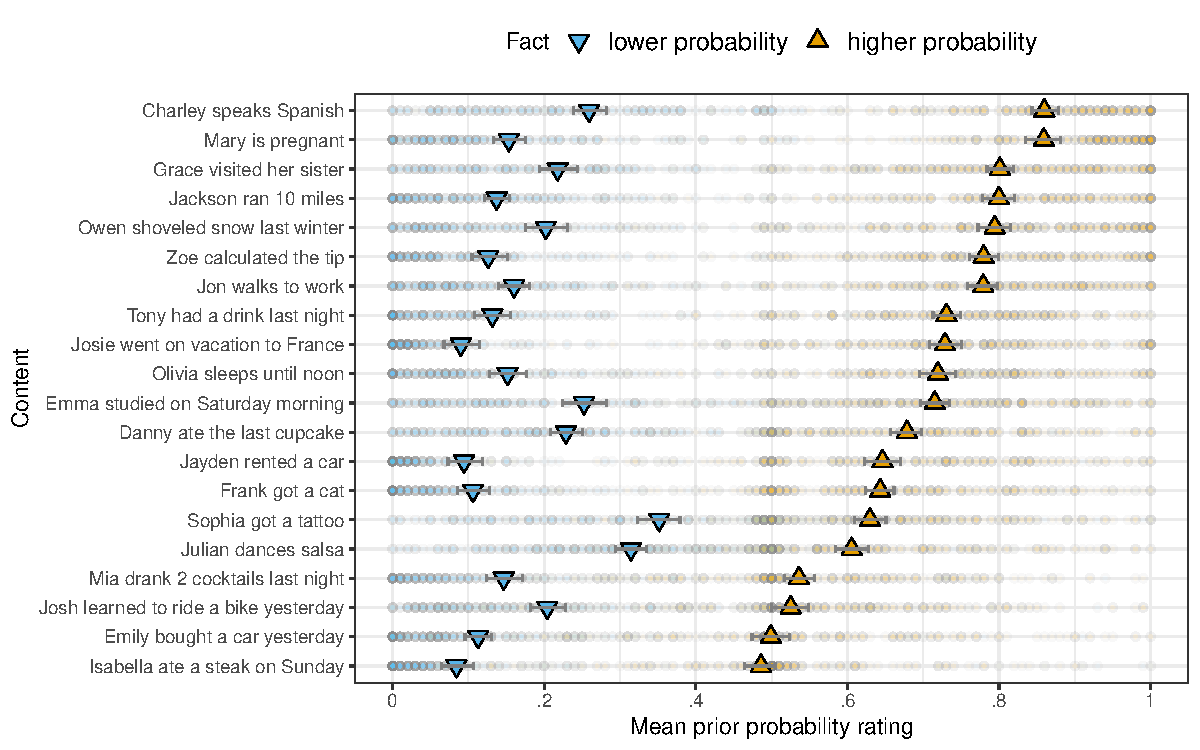
\includegraphics[width=.7\paperwidth]{../../results/exp1/graphs/prior-ratings}

\caption{Mean prior probability rating by content and fact in Exp.~1. Error bars indicate 95\% bootstrapped confidence intervals. Transparent dots indicate individual participant ratings.} 
\label{f-prior}
\end{figure}

\newpage

\section{Exp.~1: Results by block order}\label{a-blockOrderExp1}

The figures in this section present the results of Exp.~1 by block order, with the results for the two blocks side-by-side.

\subsection{Exp.~1: Certainty against prior probability ratings, by block order}

\begin{figure}[h!]
\centering
\begin{subfigure}[t]{0.49\textwidth}
\centering
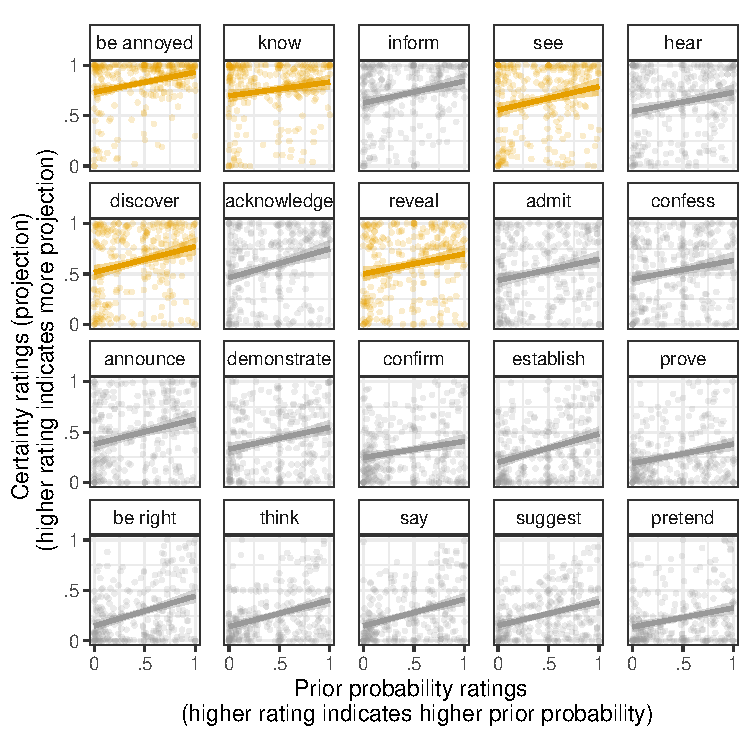
\includegraphics[width=.9\textwidth]{../../results/exp1/graphs/SUP-projai-projection-by-prior}
\caption{Proj/ai dataset.}
\end{subfigure} \hfill \begin{subfigure}[t]{0.49\textwidth}
\centering
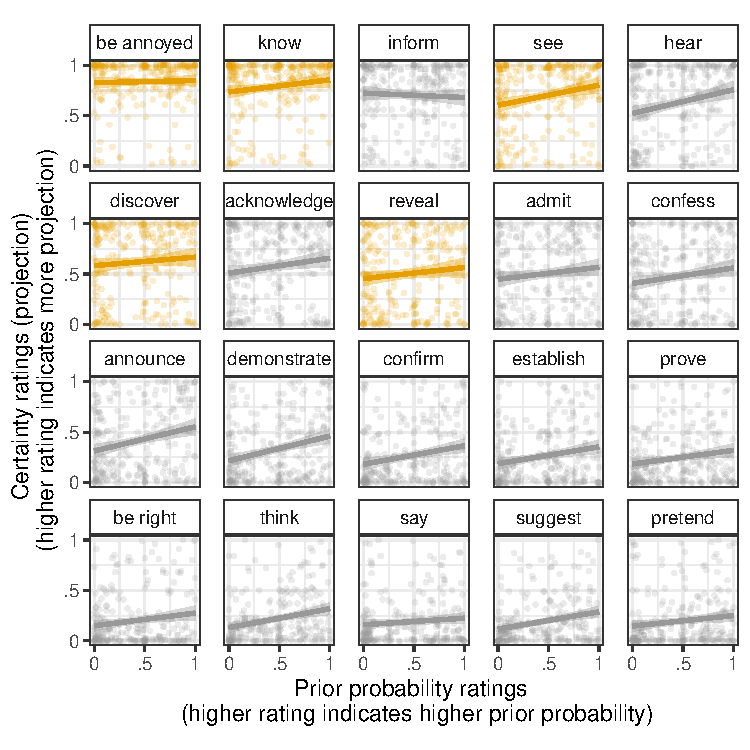
\includegraphics[width=.9\textwidth]{../../results/exp1/graphs/SUP-aiproj-projection-by-prior}
\caption{Ai/proj dataset.}
 \end{subfigure}
 
  
\caption{Participants' certainty ratings (measuring projection) against prior probability ratings in Exp.~2: (a) Proj/ai dataset, (b) Ai/proj dataset. Linear smoothers with 95\% confidence intervals overlaid. Predicates are ordered by projection mean, with purportedly factive predicates in orange.}
\end{figure}

\newpage

\subsection{Exp.~1: Certainty against asking-whether ratings, by block order}

\begin{figure}[h!]
\centering
\begin{subfigure}[t]{0.49\textwidth}
\centering
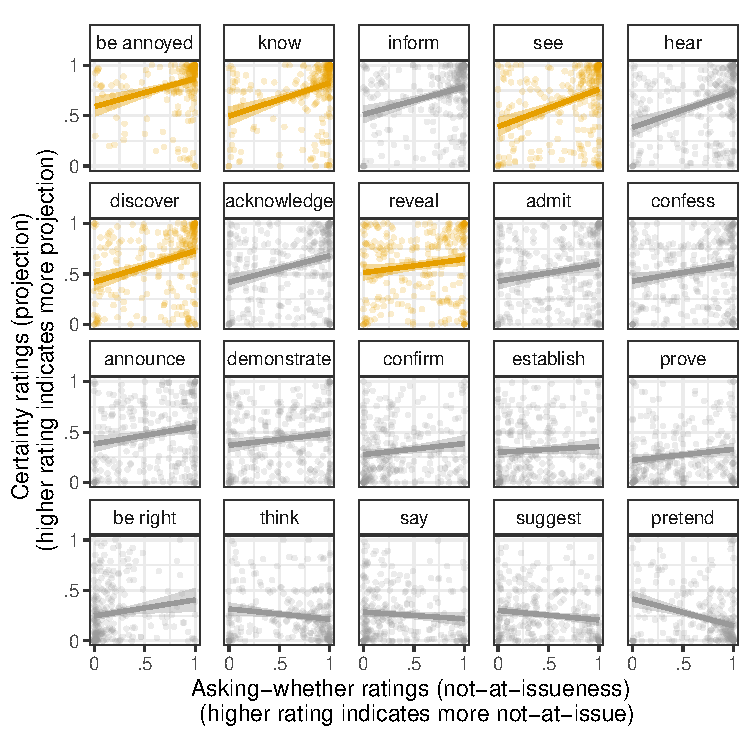
\includegraphics[width=.9\textwidth]{../../results/exp1/graphs/SUP-projai-projection-by-ai}
\caption{Proj/ai dataset.}
\end{subfigure} \hfill \begin{subfigure}[t]{0.49\textwidth}
\centering
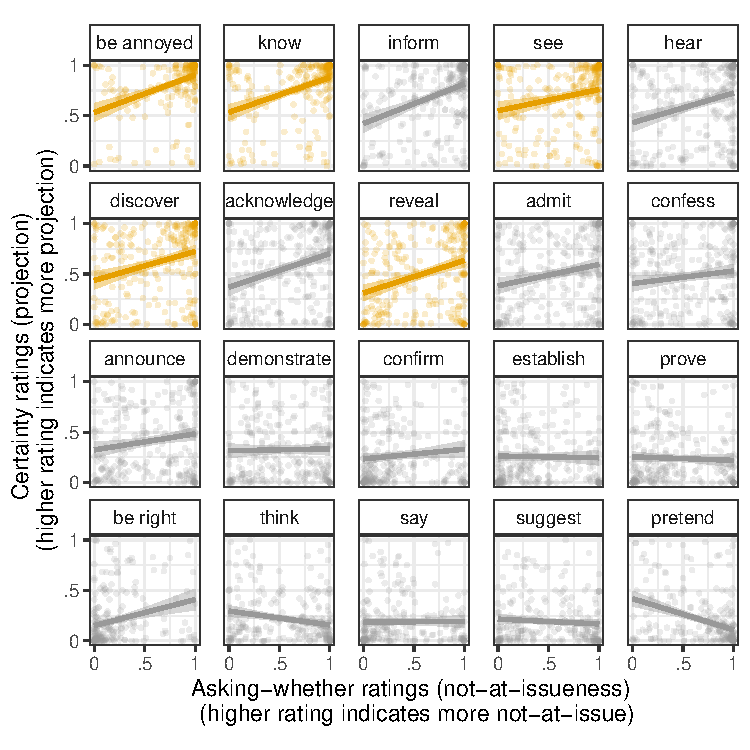
\includegraphics[width=.9\textwidth]{../../results/exp1/graphs/SUP-aiproj-projection-by-ai}
\caption{Ai/proj dataset.}
 \end{subfigure}
 
  
\caption{Participants' certainty ratings (measuring projection) against asking-whether ratings (measuring projection) in Exp.~1: (a) Proj/ai dataset, (b) Ai/proj dataset. Linear smoothers with 95\% confidence intervals overlaid. Predicates are ordered by projection mean, with purportedly factive predicates in orange.}
\end{figure}

\newpage

\subsection{Exp.~1: Certainty against asking-whether ratings by prior probability, by block order}

\begin{figure}[h!]
\centering
\begin{subfigure}[t]{0.49\textwidth}
\centering
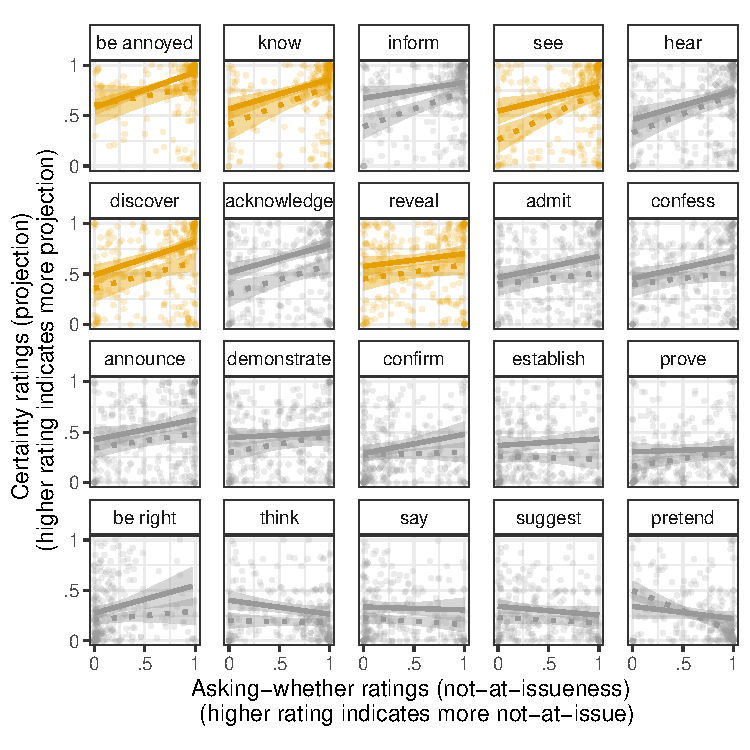
\includegraphics[width=.9\textwidth]{../../results/exp1/graphs/SUP-projai-projection-by-ai-and-prior}
\caption{Proj/ai dataset.}
\end{subfigure} \hfill \begin{subfigure}[t]{0.49\textwidth}
\centering
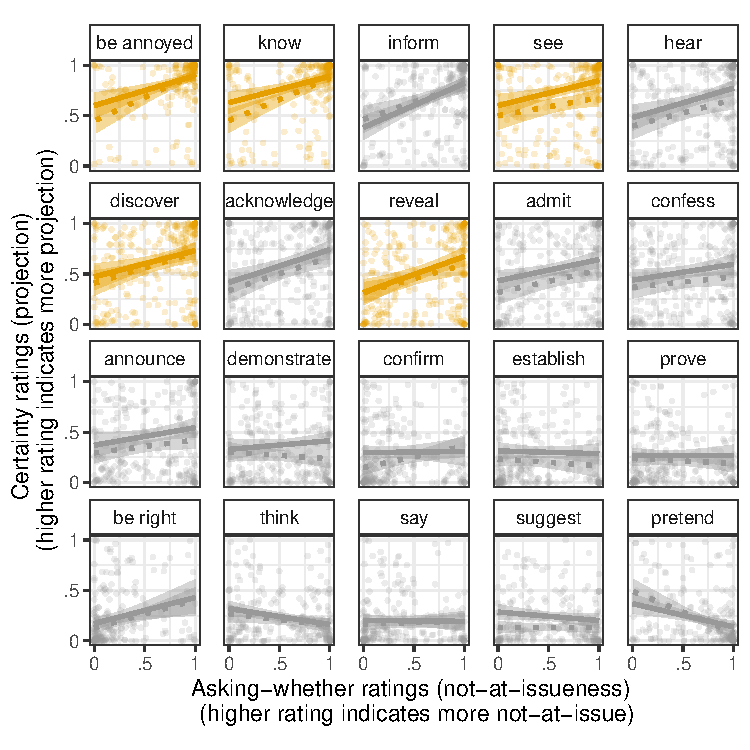
\includegraphics[width=.9\textwidth]{../../results/exp1/graphs/SUP-aiproj-projection-by-ai-and-prior}
\caption{Ai/proj dataset.}
 \end{subfigure}
 
  
\caption{Participants' certainty ratings (measuring projection) against asking-whether ratings (measuring at-issueness) by high (solid line: ---) and low prior probability fact (dotted line: \raisebox{1mm}{\ldots}) in Exp.~1: (a) Proj/ai dataset, (b) Ai/proj dataset. Linear smoothers with 95\% confidence intervals overlaid Predicates are ordered by projection mean, with purportedly factive predicates in orange.}
\end{figure}

\newpage

\subsection{Exp.~1: Asking-whether against prior probability ratings, by block order}

\begin{figure}[h!]
\centering
\begin{subfigure}[t]{0.49\textwidth}
\centering
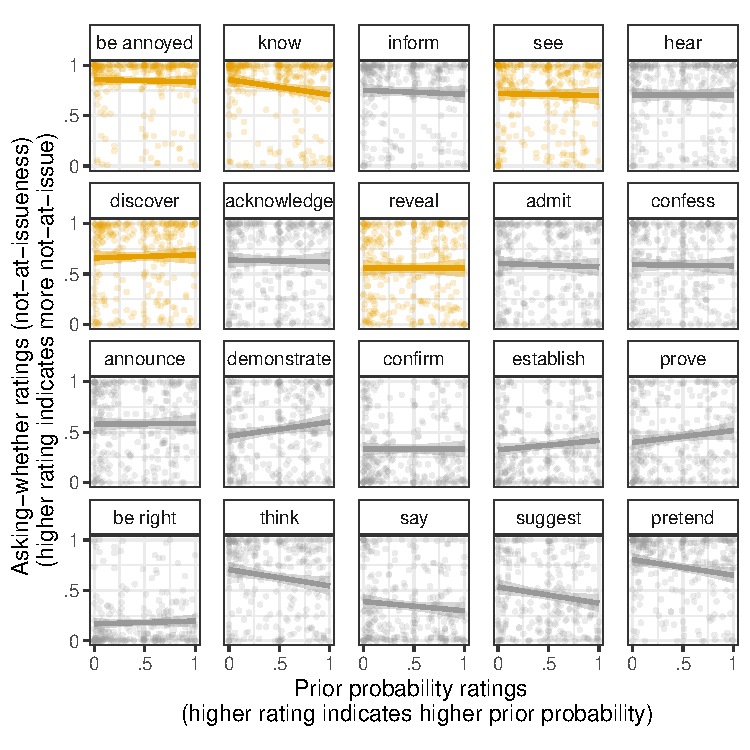
\includegraphics[width=.9\textwidth]{../../results/exp1/graphs/SUP-projai-ai-by-prior}
\caption{Proj/ai dataset.}
\end{subfigure} \hfill \begin{subfigure}[t]{0.49\textwidth}
\centering
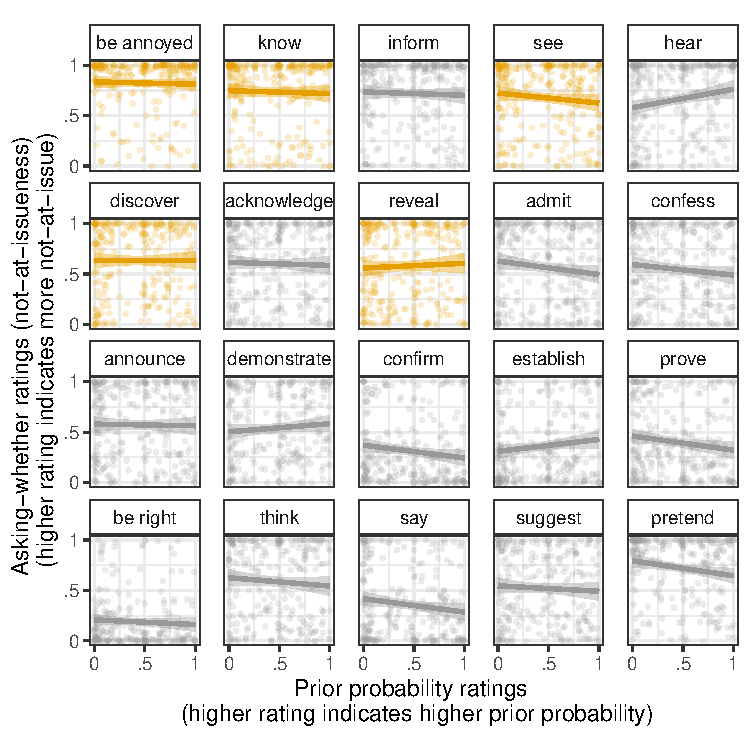
\includegraphics[width=.9\textwidth]{../../results/exp1/graphs/SUP-aiproj-ai-by-prior}
\caption{Ai/proj dataset.}
 \end{subfigure}
 
  
\caption{Participants' asking-whether ratings (measuring at-issueness) against prior probability ratings in Exp.~1: (a) Proj/ai dataset, (b) Ai/proj dataset. Linear smoothers with 95\% confidence intervals overlaid. Predicates are ordered by projection mean, with purportedly factive predicates in orange.}
\end{figure}

\newpage

\section{Exp.~2: Results by block order}\label{a-blockOrderExp2}

The figures in this section present the results of Exp.~2 by block order, with the results for the two blocks side-by-side.

\subsection{Exp.~2: Certainty against mean prior probability ratings, by block order}

\begin{figure}[h!]
\centering
\begin{subfigure}[t]{0.49\textwidth}
\centering
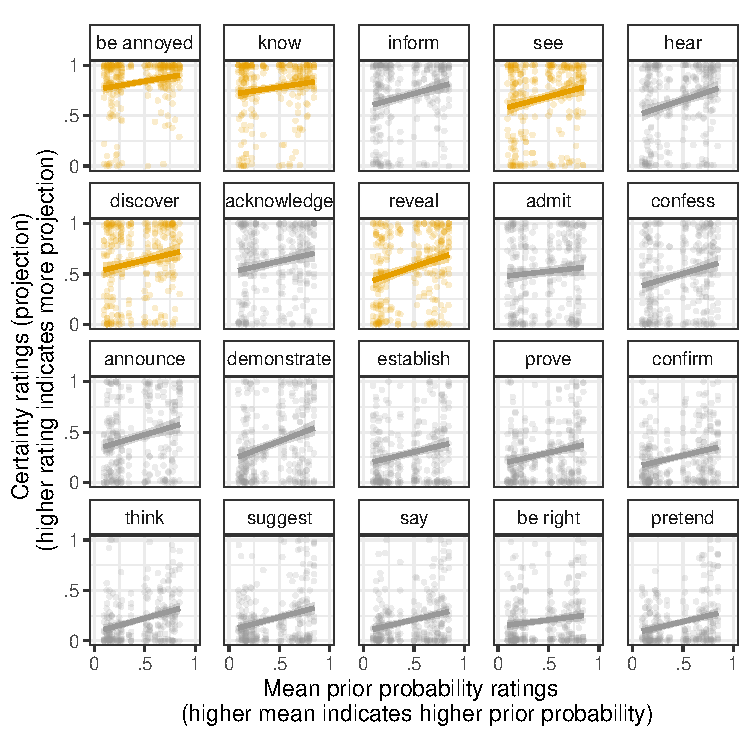
\includegraphics[width=.9\textwidth]{../../results/exp2/graphs/SUP-projai-projection-by-prior}
\caption{Proj/ai dataset.}
\end{subfigure} \hfill \begin{subfigure}[t]{0.49\textwidth}
\centering
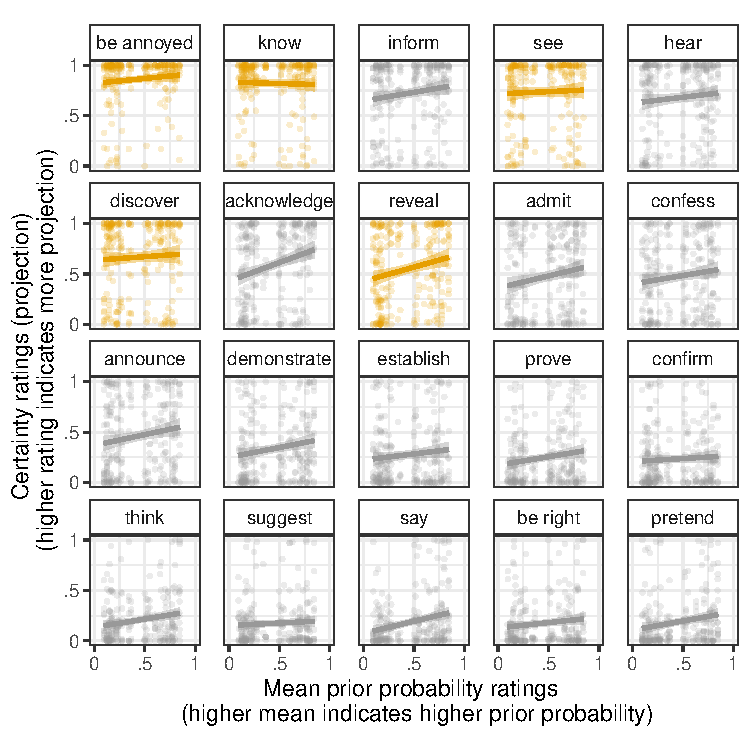
\includegraphics[width=.9\textwidth]{../../results/exp2/graphs/SUP-aiproj-projection-by-prior}
\caption{Ai/proj dataset.}
 \end{subfigure}
 
  
\caption{Participants' certainty ratings (measuring projection) against mean prior probability ratings in Exp.~2: (a) Proj/ai dataset, (b) Ai/proj dataset. Linear smoothers with 95\% confidence intervals overlaid. Predicates are ordered by projection mean, with purportedly factive predicates in orange.}
\end{figure}

\newpage

\subsection{Exp.~2: Certainty against asking-whether ratings, by block order}

\begin{figure}[h!]
\centering
\begin{subfigure}[t]{0.49\textwidth}
\centering
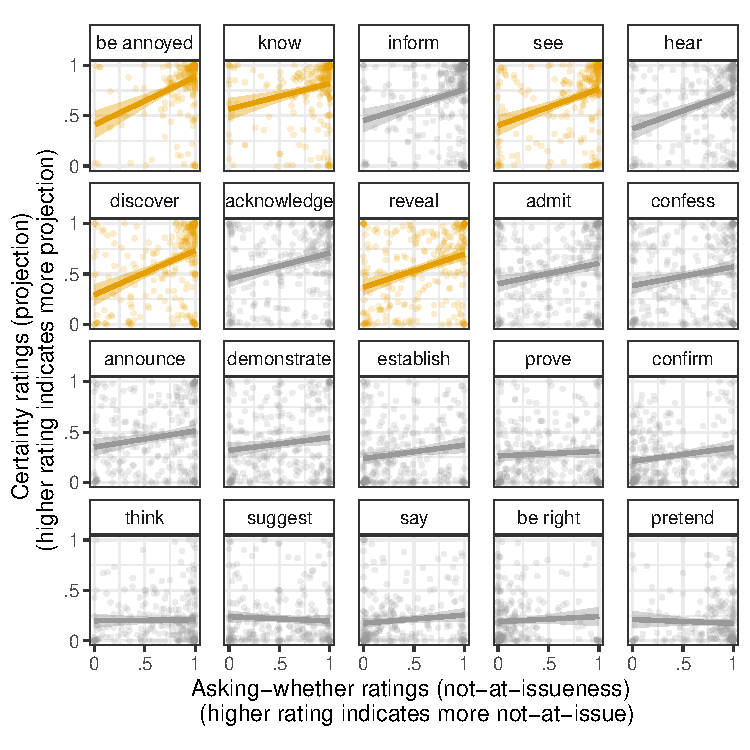
\includegraphics[width=.9\textwidth]{../../results/exp2/graphs/SUP-projai-projection-by-ai}
\caption{Proj/ai dataset.}
\end{subfigure} \hfill \begin{subfigure}[t]{0.49\textwidth}
\centering
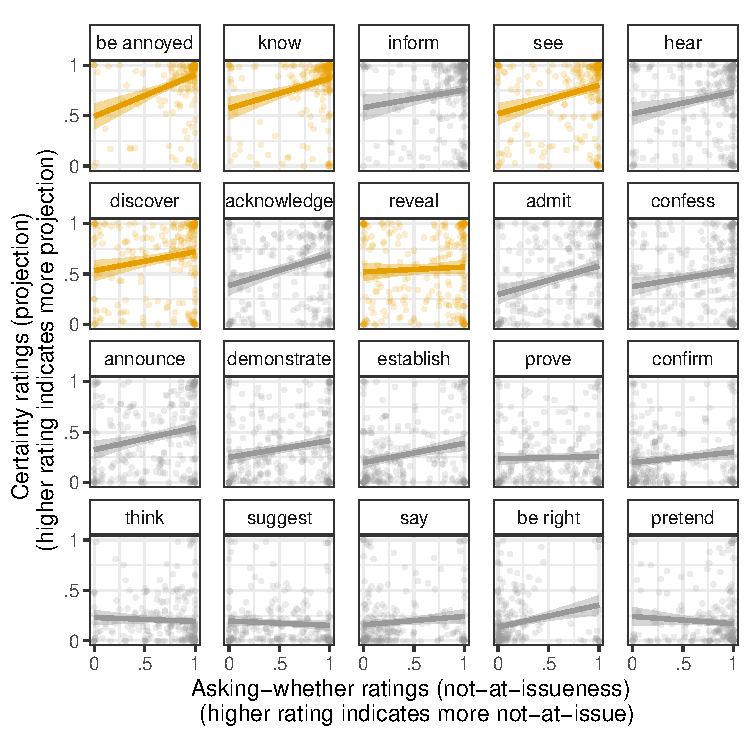
\includegraphics[width=.9\textwidth]{../../results/exp2/graphs/SUP-aiproj-projection-by-ai}
\caption{Ai/proj dataset.}
 \end{subfigure}
 
  
\caption{Participants' certainty ratings (measuring projection) against asking-whether ratings (measuring projection) in Exp.~2: (a) Proj/ai dataset, (b) Ai/proj dataset. Linear smoothers with 95\% confidence intervals overlaid. Predicates are ordered by projection mean, with purportedly factive predicates in orange.}
\end{figure}

\newpage

\subsection{Exp.~2: Certainty against asking-whether ratings by prior probability, by block order}

\begin{figure}[h!]
\centering
\begin{subfigure}[t]{0.49\textwidth}
\centering
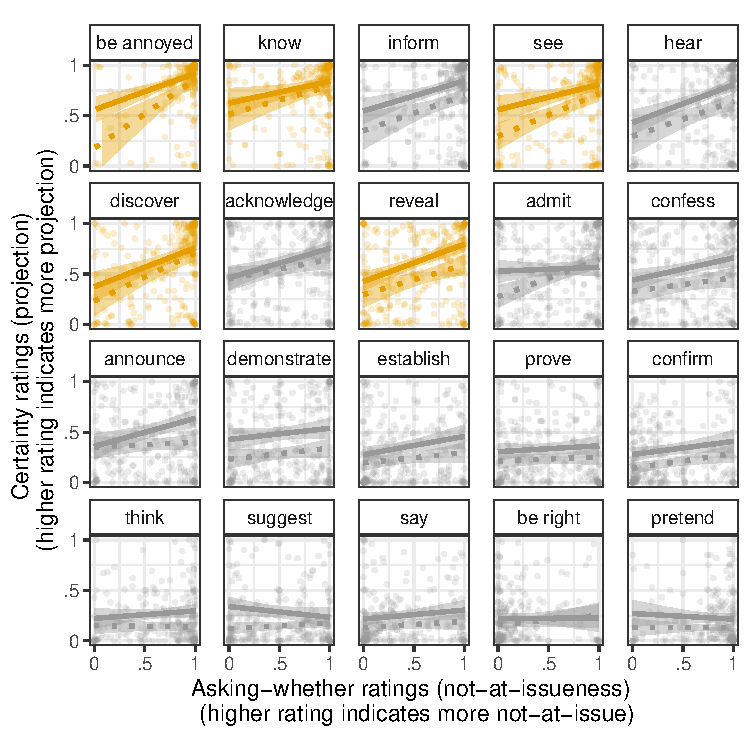
\includegraphics[width=.9\textwidth]{../../results/exp2/graphs/SUP-projai-projection-by-ai-and-prior}
\caption{Proj/ai dataset.}
\end{subfigure} \hfill \begin{subfigure}[t]{0.49\textwidth}
\centering
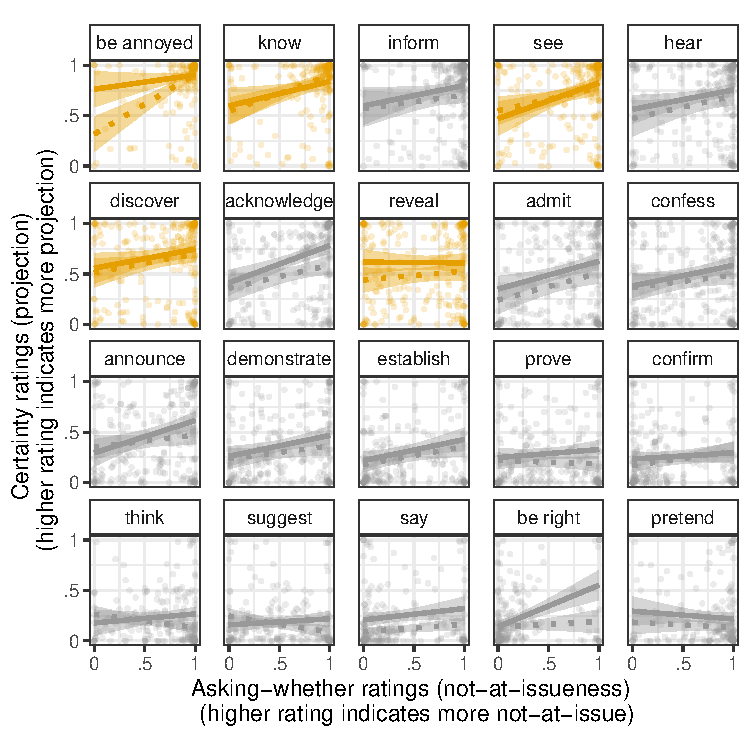
\includegraphics[width=.9\textwidth]{../../results/exp2/graphs/SUP-aiproj-projection-by-ai-and-prior}
\caption{Ai/proj dataset.}
 \end{subfigure}
 
  
\caption{Participants' certainty ratings (measuring projection) against asking-whether ratings (measuring at-issueness) by high (solid line: ---) and low prior probability fact (dotted line: \raisebox{1mm}{\ldots}) in Exp.~1: (a) Proj/ai dataset, (b) Ai/proj dataset. Linear smoothers with 95\% confidence intervals overlaid Predicates are ordered by projection mean, with purportedly factive predicates in orange.}
\end{figure}

\newpage

\subsection{Exp.~2: Asking-whether against prior probability ratings, by block order}

\begin{figure}[h!]
\centering
\begin{subfigure}[t]{0.49\textwidth}
\centering
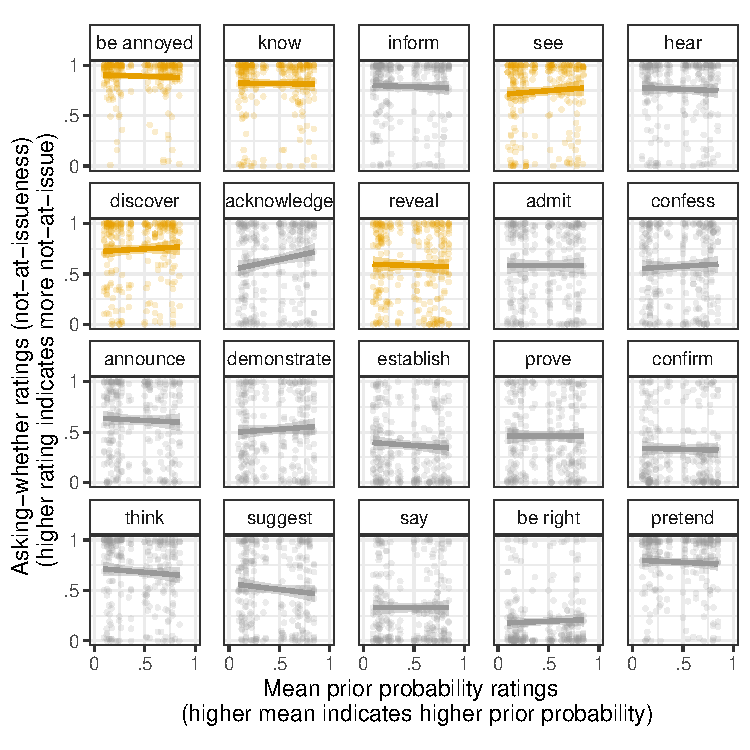
\includegraphics[width=.9\textwidth]{../../results/exp2/graphs/SUP-projai-ai-by-prior}
\caption{Proj/ai dataset.}
\end{subfigure} \hfill \begin{subfigure}[t]{0.49\textwidth}
\centering
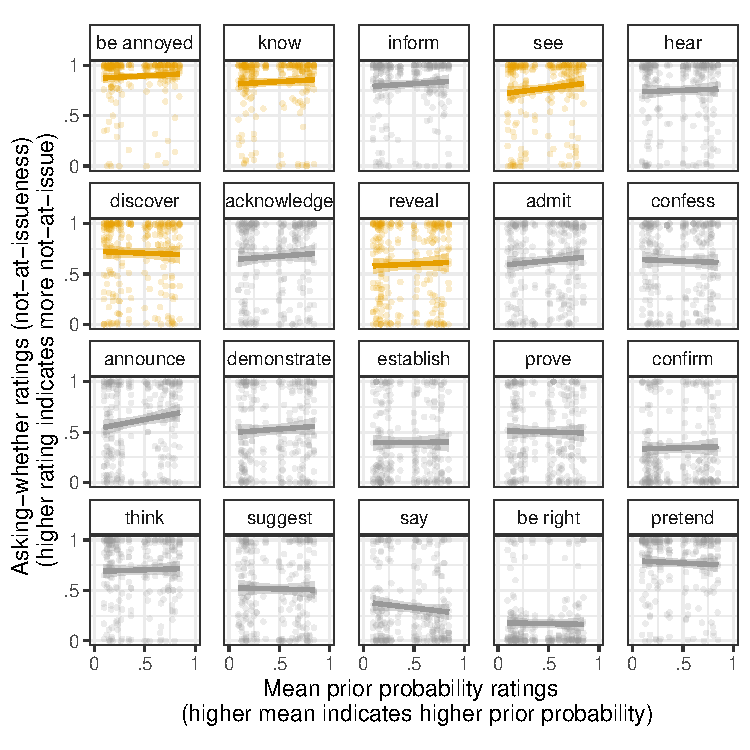
\includegraphics[width=.9\textwidth]{../../results/exp2/graphs/SUP-aiproj-ai-by-prior}
\caption{Ai/proj dataset.}
 \end{subfigure}
 
  
\caption{Participants' asking-whether ratings (measuring at-issueness) against mean prior probability ratings in Exp.~2: (a) Proj/ai dataset, (b) Ai/proj dataset. Linear smoothers with 95\% confidence intervals overlaid. Predicates are ordered by projection mean, with purportedly factive predicates in orange.}
\end{figure}

\newpage

\section{By-predicate mean projection against mean not-at-issueness}\label{a-proj-by-ai}

\begin{figure}[h!]
\centering
\begin{subfigure}[t]{.49\textwidth}
\centering
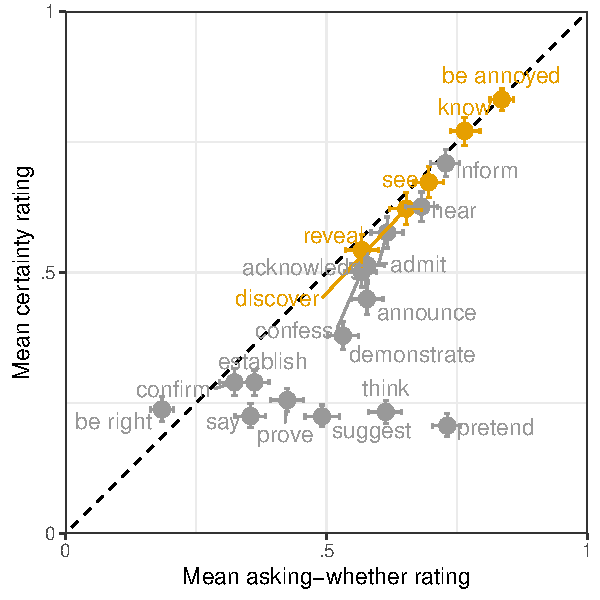
\includegraphics[width=\textwidth]{../../results/exp1/graphs/SUP-mean-projection-by-mean-ai}
\caption{Exp.~1}\label{fig:prior-exp1-expDT1}
\end{subfigure} \hfill \begin{subfigure}[t]{.49\textwidth}
\centering
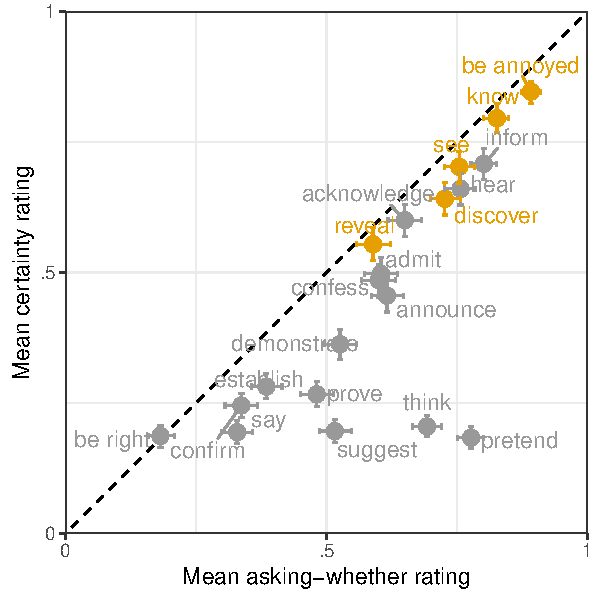
\includegraphics[width=\textwidth]{../../results/exp2/graphs/SUP-mean-projection-by-mean-ai}
\caption{Exp.~2}\label{}
 \end{subfigure}
\caption{By-predicate mean projection against mean at-issueness. Purportedly factive predicates in orange. Error bars indicate 95\% bootstrapped confidence intervals.}\label{fig:SUP-proj-by-ai}
\end{figure}

\newpage

\section{Cross-experiment comparisons of ratings}\label{a-replication}

\subsection{Prior belief ratings}

Fig.~\ref{fig:SUP-prior-comparison} compares the mean by-content/fact prior probability ratings from Exp.~1 and the two experiments in \citealt{degen-tonhauser-openmind} (referred to as DT1 and DT2). For each content/fact combination, there was a mean of 252 ratings in Exp.~1, a mean of 143 ratings in DT1, and a mean of 38 ratings in DT2.

\begin{figure}[h!]
\centering
\begin{subfigure}[t]{.3\textwidth}
\centering
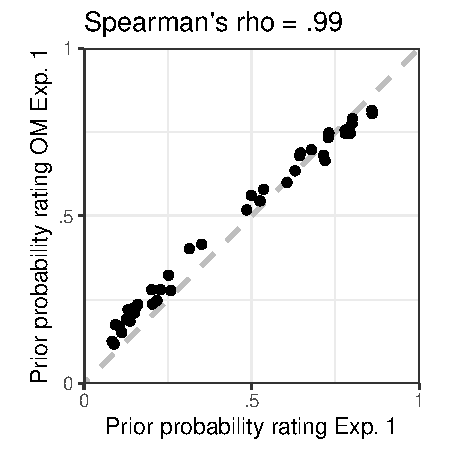
\includegraphics[width=\textwidth]{../../results/exp1/graphs/SUP-priorExp1-by-priorOMExp1}
\caption{Exp.~DT1 against Exp.~1}\label{fig:prior-exp1-expDT1}
\end{subfigure} \hfill \begin{subfigure}[t]{.3\textwidth}
\centering
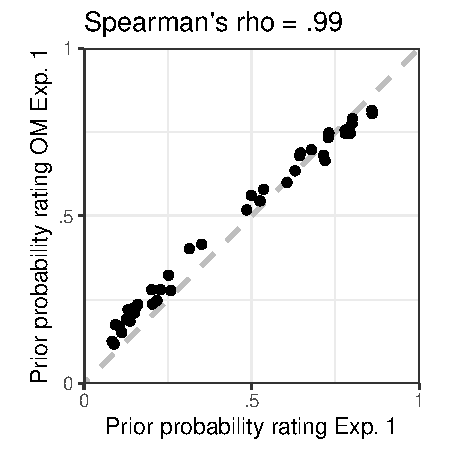
\includegraphics[width=\textwidth]{../../results/exp1/graphs/SUP-priorExp1-by-priorOMExp1}
\caption{Exp.~DT2 against Exp.~1.}\label{fig:prior-exp1-expDT2a}
 \end{subfigure} \hfill \begin{subfigure}[t]{.3\textwidth}
\centering
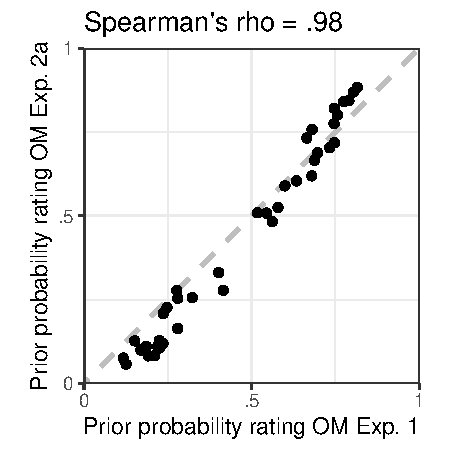
\includegraphics[width=\textwidth]{../../results/exp1/graphs/SUP-priorOMExp1-by-priorOMExp2a}
\caption{Exp.~DT2 against Exp.~DT1}\label{fig:prior-expDT1-expDT2a}
 \end{subfigure}
\caption{Comparisons of 40 mean by-content/fact prior belief ratings in Exp.~1 and the two experiments in \citealt{degen-tonhauser-openmind} (abbreviated DT1 and DT2), with Spearman rank effects in the title. Error bars indicate 95\% bootstrapped confidence intervals.}\label{fig:SUP-prior-comparison}
\end{figure}

\subsection{Certain-that ratings (projection)}

Fig.~\ref{fig:SUP-certainty-comparison} compares the certainty ratings from Exps.~1 and 2. For each predicate, there were 505 ratings in Exp.~1 and 500 ratings in Exp.~2. For each predicate/content combination, there was a mean of 25 ratings in both Exps.~1 and 2. For each predicate/content/fact combination, there was a mean of 13 ratings in both Exps.~1 and 2.

\begin{figure}[h!]
\centering
\begin{subfigure}[t]{.3\textwidth}
\centering
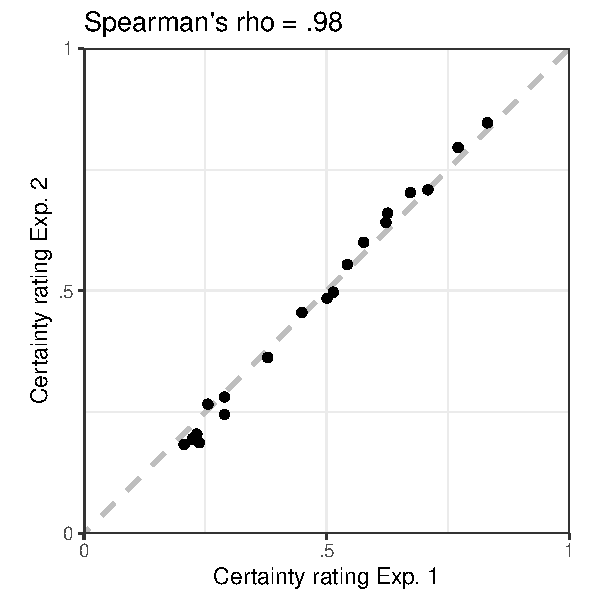
\includegraphics[width=\textwidth]{../../results/exp1/graphs/SUP-certainty-Exp1-by-Exp2}
\caption{By-predicate means}
 \end{subfigure}\hfill
\begin{subfigure}[t]{.3\textwidth}
\centering
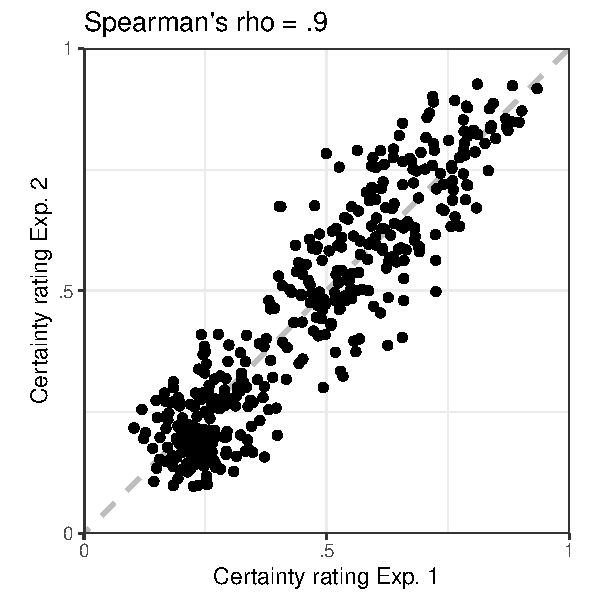
\includegraphics[width=\textwidth]{../../results/exp1/graphs/SUP-certainty-PredItem-Exp1-by-Exp2}
\caption{By-predicate/item means}
\end{subfigure}\hfill
\begin{subfigure}[t]{.3\textwidth}
\centering
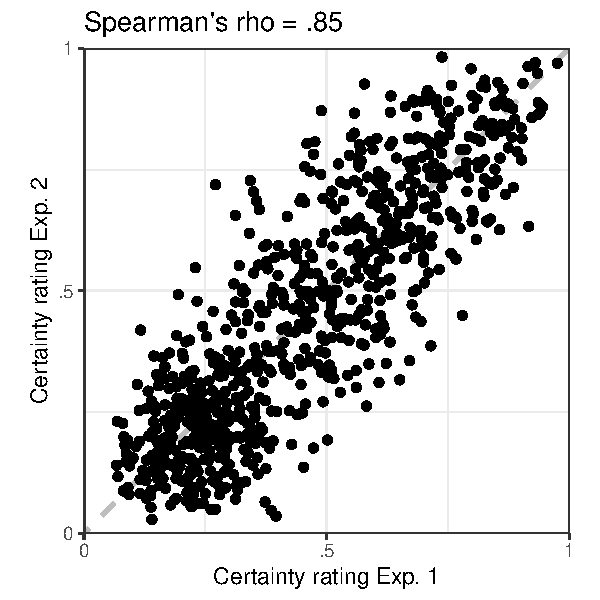
\includegraphics[width=\textwidth]{../../results/exp1/graphs/SUP-certainty-PredItemFact-Exp1-by-Exp2}
\caption{By-predicate/item/fact means}
\end{subfigure}  
\caption{Comparisons of (a) 20 mean by-predicate, (b) 400 by-predicate/item certainty ratings, and (c) 800 by-predicate/item certainty ratings from Exps.~1 and 2,  with Spearman rank effects in the title. Error bars indicate 95\% bootstrapped confidence intervals.}\label{fig:SUP-certainty-comparison}
\end{figure}

\newpage

\subsection{Asking-whether ratings (at-issueness)}

Fig.~\ref{fig:SUP-ai-comparison} compares the certainty ratings from Exps.~1 and 2. For each predicate, there were 505 ratings in Exp.~1 and 500 ratings in Exp.~2. For each predicate/content combination, there was a mean of 25 ratings in both Exps.~1 and 2. For each predicate/content/fact combination, there was a mean of 13 ratings in both Exps.~1 and 2.

\begin{figure}[h!]
\centering
\begin{subfigure}[t]{.3\textwidth}
\centering
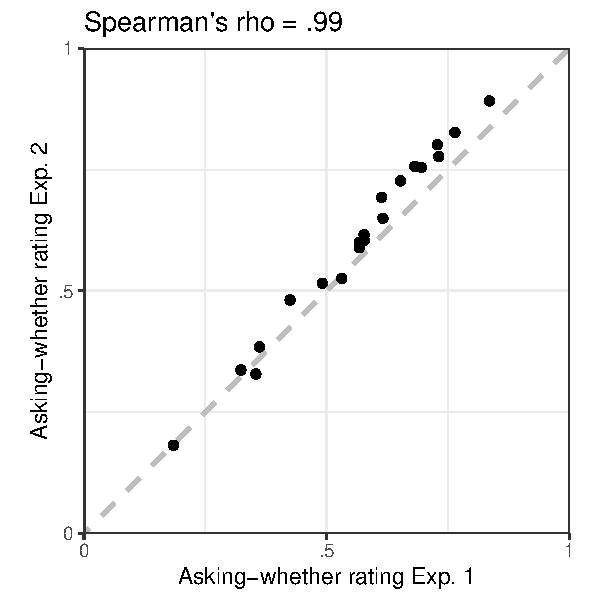
\includegraphics[width=\textwidth]{../../results/exp1/graphs/SUP-ai-Exp1-by-Exp2}
\caption{By-predicate means}
 \end{subfigure}\hfill
\begin{subfigure}[t]{.3\textwidth}
\centering
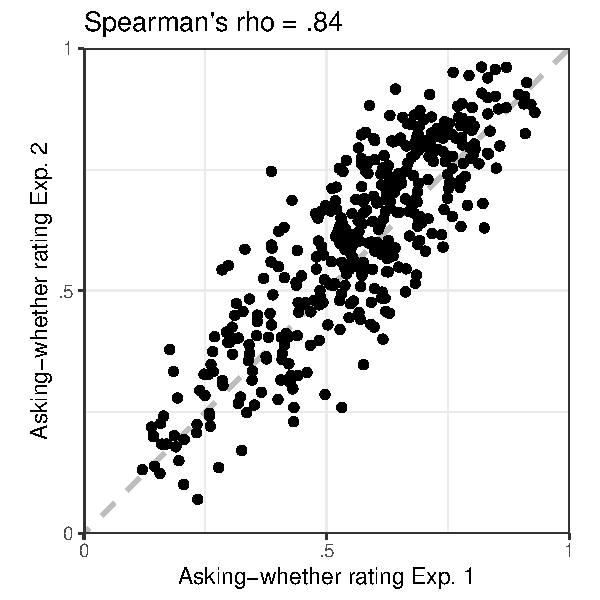
\includegraphics[width=\textwidth]{../../results/exp1/graphs/SUP-ai-PredItem-Exp1-by-Exp2}
\caption{By-predicate/item means}
\end{subfigure}\hfill
\begin{subfigure}[t]{.3\textwidth}
\centering
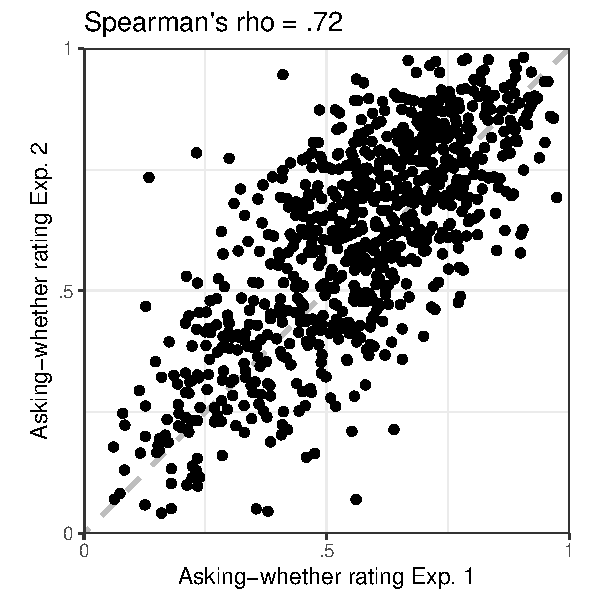
\includegraphics[width=\textwidth]{../../results/exp1/graphs/SUP-ai-PredItemFact-Exp1-by-Exp2}
\caption{By-predicate/item/fact means}
\end{subfigure}  
\caption{Comparisons of (a) 20 mean by-predicate, (b) 400 by-predicate/item certainty ratings, and (c) 800 by-predicate/item asking-whether ratings from Exps.~1 and 2,  with Spearman rank effects in the title. Error bars indicate 95\% bootstrapped confidence intervals.}\label{fig:SUP-ai-comparison}
\end{figure}
\end{document}


